%DIF LATEXDIFF DIFFERENCE FILE


%% bare_jrnl_compsoc.tex
%% V1.4b
%% 2015/08/26
%% by Michael Shell
%% See:
%% http://www.michaelshell.org/
%% for current contact information.
%%
%% This is a skeleton file demonstrating the use of IEEEtran.cls
%% (requires IEEEtran.cls version 1.8b or later) with an IEEE
%% Computer Society journal paper.
%%
%% Support sites:
%% http://www.michaelshell.org/tex/ieeetran/
%% http://www.ctan.org/pkg/ieeetran
%% and
%% http://www.ieee.org/

%%*************************************************************************
%% Legal Notice:
%% This code is offered as-is without any warranty either expressed or
%% implied; without even the implied warranty of MERCHANTABILITY or
%% FITNESS FOR A PARTICULAR PURPOSE! 
%% User assumes all risk.
%% In no event shall the IEEE or any contributor to this code be liable for
%% any damages or losses, including, but not limited to, incidental,
%% consequential, or any other damages, resulting from the use or misuse
%% of any information contained here.
%%
%% All comments are the opinions of their respective authors and are not
%% necessarily endorsed by the IEEE.
%%
%% This work is distributed under the LaTeX Project Public License (LPPL)
%% ( http://www.latex-project.org/ ) version 1.3, and may be freely used,
%% distributed and modified. A copy of the LPPL, version 1.3, is included
%% in the base LaTeX documentation of all distributions of LaTeX released
%% 2003/12/01 or later.
%% Retain all contribution notices and credits.
%% ** Modified files should be clearly indicated as such, including  **
%% ** renaming them and changing author support contact information. **
%%*************************************************************************


% *** Authors should verify (and, if needed, correct) their LaTeX system  ***
% *** with the testflow diagnostic prior to trusting their LaTeX platform ***
% *** with production work. The IEEE's font choices and paper sizes can   ***
% *** trigger bugs that do not appear when using other class files.       ***                          ***
% The testflow support page is at:
% http://www.michaelshell.org/tex/testflow/


\documentclass[10pt,journal,compsoc]{IEEEtran}
\usepackage{graphicx}
\usepackage{stfloats}
\usepackage[nocompress]{cite}
\usepackage{amsmath}
\usepackage{cases}
\usepackage{algorithmic}
\usepackage[caption=false,font=footnotesize,labelfont=sf,textfont=sf]{subfig}
%DIF 61a61-62
\usepackage{xcolor} %DIF > 
\usepackage{amsfonts} %DIF > 
%DIF -------
%\usepackage[T1]{fontenc}%加粗有效
%
% If IEEEtran.cls has not been installed into the LaTeX system files,
% manually specify the path to it like:
% \documentclass[10pt,journal,compsoc]{../sty/IEEEtran}





% Some very useful LaTeX packages include:
% (uncomment the ones you want to load)


% *** MISC UTILITY PACKAGES ***
%
%\usepackage{ifpdf}
% Heiko Oberdiek's ifpdf.sty is very useful if you need conditional
% compilation based on whether the output is pdf or dvi.
% usage:
% \ifpdf
%   % pdf code
% \else
%   % dvi code
% \fi
% The latest version of ifpdf.sty can be obtained from:
% http://www.ctan.org/pkg/ifpdf
% Also, note that IEEEtran.cls V1.7 and later provides a builtin
% \ifCLASSINFOpdf conditional that works the same way.
% When switching from latex to pdflatex and vice-versa, the compiler may
% have to be run twice to clear warning/error messages.






% *** CITATION PACKAGES ***
%
%\ifCLASSOPTIONcompsoc
%  % IEEE Computer Society needs nocompress option
%  % requires cite.sty v4.0 or later (November 2003)
%  \usepackage[nocompress]{cite}
%\else
%  % normal IEEE
%  \usepackage{cite}
%\fi
% cite.sty was written by Donald Arseneau
% V1.6 and later of IEEEtran pre-defines the format of the cite.sty package
% \cite{} output to follow that of the IEEE. Loading the cite package will
% result in citation numbers being automatically sorted and properly
% "compressed/ranged". e.g., [1], [9], [2], [7], [5], [6] without using
% cite.sty will become [1], [2], [5]--[7], [9] using cite.sty. cite.sty's
% \cite will automatically add leading space, if needed. Use cite.sty's
% noadjust option (cite.sty V3.8 and later) if you want to turn this off
% such as if a citation ever needs to be enclosed in parenthesis.
% cite.sty is already installed on most LaTeX systems. Be sure and use
% version 5.0 (2009-03-20) and later if using hyperref.sty.
% The latest version can be obtained at:
% http://www.ctan.org/pkg/cite
% The documentation is contained in the cite.sty file itself.
%
% Note that some packages require special options to format as the Computer
% Society requires. In particular, Computer Society  papers do not use
% compressed citation ranges as is done in typical IEEE papers
% (e.g., [1]-[4]). Instead, they list every citation separately in order
% (e.g., [1], [2], [3], [4]). To get the latter we need to load the cite
% package with the nocompress option which is supported by cite.sty v4.0
% and later. Note also the use of a CLASSOPTION conditional provided by
% IEEEtran.cls V1.7 and later.





% *** GRAPHICS RELATED PACKAGES ***
%
\ifCLASSINFOpdf
% \usepackage[pdftex]{graphicx}
% declare the path(s) where your graphic files are
% \graphicspath{{../pdf/}{../jpeg/}}
% and their extensions so you won't have to specify these with
% every instance of \includegraphics
% \DeclareGraphicsExtensions{.pdf,.jpeg,.png}
\else
% or other class option (dvipsone, dvipdf, if not using dvips). graphicx
% will default to the driver specified in the system graphics.cfg if no
% driver is specified.
% \usepackage[dvips]{graphicx}
% declare the path(s) where your graphic files are
% \graphicspath{{../eps/}}
% and their extensions so you won't have to specify these with
% every instance of \includegraphics
% \DeclareGraphicsExtensions{.eps}
\fi
% graphicx was written by David Carlisle and Sebastian Rahtz. It is
% required if you want graphics, photos, etc. graphicx.sty is already
% installed on most LaTeX systems. The latest version and documentation
% can be obtained at: 
% http://www.ctan.org/pkg/graphicx
% Another good source of documentation is "Using Imported Graphics in
% LaTeX2e" by Keith Reckdahl which can be found at:
% http://www.ctan.org/pkg/epslatex
%
% latex, and pdflatex in dvi mode, support graphics in encapsulated
% postscript (.eps) format. pdflatex in pdf mode supports graphics
% in .pdf, .jpeg, .png and .mps (metapost) formats. Users should ensure
% that all non-photo figures use a vector format (.eps, .pdf, .mps) and
% not a bitmapped formats (.jpeg, .png). The IEEE frowns on bitmapped formats
% which can result in "jaggedy"/blurry rendering of lines and letters as
% well as large increases in file sizes.
%
% You can find documentation about the pdfTeX application at:
% http://www.tug.org/applications/pdftex






% *** MATH PACKAGES ***
%
%\usepackage{amsmath}
% A popular package from the American Mathematical Society that provides
% many useful and powerful commands for dealing with mathematics.
%
% Note that the amsmath package sets \interdisplaylinepenalty to 10000
% thus preventing page breaks from occurring within multiline equations. Use:
%\interdisplaylinepenalty=2500
% after loading amsmath to restore such page breaks as IEEEtran.cls normally
% does. amsmath.sty is already installed on most LaTeX systems. The latest
% version and documentation can be obtained at:
% http://www.ctan.org/pkg/amsmath





% *** SPECIALIZED LIST PACKAGES ***
%
%\usepackage{algorithmic}
% algorithmic.sty was written by Peter Williams and Rogerio Brito.
% This package provides an algorithmic environment fo describing algorithms.
% You can use the algorithmic environment in-text or within a figure
% environment to provide for a floating algorithm. Do NOT use the algorithm
% floating environment provided by algorithm.sty (by the same authors) or
% algorithm2e.sty (by Christophe Fiorio) as the IEEE does not use dedicated
% algorithm float types and packages that provide these will not provide
% correct IEEE style captions. The latest version and documentation of
% algorithmic.sty can be obtained at:
% http://www.ctan.org/pkg/algorithms
% Also of interest may be the (relatively newer and more customizable)
% algorithmicx.sty package by Szasz Janos:
% http://www.ctan.org/pkg/algorithmicx




% *** ALIGNMENT PACKAGES ***
%
%\usepackage{array}
% Frank Mittelbach's and David Carlisle's array.sty patches and improves
% the standard LaTeX2e array and tabular environments to provide better
% appearance and additional user controls. As the default LaTeX2e table
% generation code is lacking to the point of almost being broken with
% respect to the quality of the end results, all users are strongly
% advised to use an enhanced (at the very least that provided by array.sty)
% set of table tools. array.sty is already installed on most systems. The
% latest version and documentation can be obtained at:
% http://www.ctan.org/pkg/array


% IEEEtran contains the IEEEeqnarray family of commands that can be used to
% generate multiline equations as well as matrices, tables, etc., of high
% quality.




% *** SUBFIGURE PACKAGES ***
%\ifCLASSOPTIONcompsoc
%  \usepackage[caption=false,font=footnotesize,labelfont=sf,textfont=sf]{subfig}
%\else
%  \usepackage[caption=false,font=footnotesize]{subfig}
%\fi
% subfig.sty, written by Steven Douglas Cochran, is the modern replacement
% for subfigure.sty, the latter of which is no longer maintained and is
% incompatible with some LaTeX packages including fixltx2e. However,
% subfig.sty requires and automatically loads Axel Sommerfeldt's caption.sty
% which will override IEEEtran.cls' handling of captions and this will result
% in non-IEEE style figure/table captions. To prevent this problem, be sure
% and invoke subfig.sty's "caption=false" package option (available since
% subfig.sty version 1.3, 2005/06/28) as this is will preserve IEEEtran.cls
% handling of captions.
% Note that the Computer Society format requires a sans serif font rather
% than the serif font used in traditional IEEE formatting and thus the need
% to invoke different subfig.sty package options depending on whether
% compsoc mode has been enabled.
%
% The latest version and documentation of subfig.sty can be obtained at:
% http://www.ctan.org/pkg/subfig




% *** FLOAT PACKAGES ***
%
%\usepackage{fixltx2e}
% fixltx2e, the successor to the earlier fix2col.sty, was written by
% Frank Mittelbach and David Carlisle. This package corrects a few problems
% in the LaTeX2e kernel, the most notable of which is that in current
% LaTeX2e releases, the ordering of single and double column floats is not
% guaranteed to be preserved. Thus, an unpatched LaTeX2e can allow a
% single column figure to be placed prior to an earlier double column
% figure.
% Be aware that LaTeX2e kernels dated 2015 and later have fixltx2e.sty's
% corrections already built into the system in which case a warning will
% be issued if an attempt is made to load fixltx2e.sty as it is no longer
% needed.
% The latest version and documentation can be found at:
% http://www.ctan.org/pkg/fixltx2e


%\usepackage{stfloats}
% stfloats.sty was written by Sigitas Tolusis. This package gives LaTeX2e
% the ability to do double column floats at the bottom of the page as well
% as the top. (e.g., "\begin{figure*}[!b]" is not normally possible in
% LaTeX2e). It also provides a command:
%\fnbelowfloat
% to enable the placement of footnotes below bottom floats (the standard
% LaTeX2e kernel puts them above bottom floats). This is an invasive package
% which rewrites many portions of the LaTeX2e float routines. It may not work
% with other packages that modify the LaTeX2e float routines. The latest
% version and documentation can be obtained at:
% http://www.ctan.org/pkg/stfloats
% Do not use the stfloats baselinefloat ability as the IEEE does not allow
% \baselineskip to stretch. Authors submitting work to the IEEE should note
% that the IEEE rarely uses double column equations and that authors should try
% to avoid such use. Do not be tempted to use the cuted.sty or midfloat.sty
% packages (also by Sigitas Tolusis) as the IEEE does not format its papers in
% such ways.
% Do not attempt to use stfloats with fixltx2e as they are incompatible.
% Instead, use Morten Hogholm'a dblfloatfix which combines the features
% of both fixltx2e and stfloats:
%
% \usepackage{dblfloatfix}
% The latest version can be found at:
% http://www.ctan.org/pkg/dblfloatfix




%\ifCLASSOPTIONcaptionsoff
%  \usepackage[nomarkers]{endfloat}
% \let\MYoriglatexcaption\caption
% \renewcommand{\caption}[2][\relax]{\MYoriglatexcaption[#2]{#2}}
%\fi
% endfloat.sty was written by James Darrell McCauley, Jeff Goldberg and 
% Axel Sommerfeldt. This package may be useful when used in conjunction with 
% IEEEtran.cls'  captionsoff option. Some IEEE journals/societies require that
% submissions have lists of figures/tables at the end of the paper and that
% figures/tables without any captions are placed on a page by themselves at
% the end of the document. If needed, the draftcls IEEEtran class option or
% \CLASSINPUTbaselinestretch interface can be used to increase the line
% spacing as well. Be sure and use the nomarkers option of endfloat to
% prevent endfloat from "marking" where the figures would have been placed
% in the text. The two hack lines of code above are a slight modification of
% that suggested by in the endfloat docs (section 8.4.1) to ensure that
% the full captions always appear in the list of figures/tables - even if
% the user used the short optional argument of \caption[]{}.
% IEEE papers do not typically make use of \caption[]'s optional argument,
% so this should not be an issue. A similar trick can be used to disable
% captions of packages such as subfig.sty that lack options to turn off
% the subcaptions:
% For subfig.sty:
% \let\MYorigsubfloat\subfloat
% \renewcommand{\subfloat}[2][\relax]{\MYorigsubfloat[]{#2}}
% However, the above trick will not work if both optional arguments of
% the \subfloat command are used. Furthermore, there needs to be a
% description of each subfigure *somewhere* and endfloat does not add
% subfigure captions to its list of figures. Thus, the best approach is to
% avoid the use of subfigure captions (many IEEE journals avoid them anyway)
% and instead reference/explain all the subfigures within the main caption.
% The latest version of endfloat.sty and its documentation can obtained at:
% http://www.ctan.org/pkg/endfloat
%
% The IEEEtran \ifCLASSOPTIONcaptionsoff conditional can also be used
% later in the document, say, to conditionally put the References on a 
% page by themselves.




% *** PDF, URL AND HYPERLINK PACKAGES ***
%
%\usepackage{url}
% url.sty was written by Donald Arseneau. It provides better support for
% handling and breaking URLs. url.sty is already installed on most LaTeX
% systems. The latest version and documentation can be obtained at:
% http://www.ctan.org/pkg/url
% Basically, \url{my_url_here}.





% *** Do not adjust lengths that control margins, column widths, etc. ***
% *** Do not use packages that alter fonts (such as pslatex).         ***
% There should be no need to do such things with IEEEtran.cls V1.6 and later.
% (Unless specifically asked to do so by the journal or conference you plan
% to submit to, of course. )


% correct bad hyphenation here
\hyphenation{op-tical net-works semi-conduc-tor}
%DIF PREAMBLE EXTENSION ADDED BY LATEXDIFF
%DIF UNDERLINE PREAMBLE %DIF PREAMBLE
\RequirePackage[normalem]{ulem} %DIF PREAMBLE
\RequirePackage{color}\definecolor{RED}{rgb}{1,0,0}\definecolor{BLUE}{rgb}{0,0,1} %DIF PREAMBLE
\providecommand{\DIFadd}[1]{{\protect\color{blue}\uwave{#1}}} %DIF PREAMBLE
\providecommand{\DIFdel}[1]{{\protect\color{red}\sout{#1}}}                      %DIF PREAMBLE
%DIF SAFE PREAMBLE %DIF PREAMBLE
\providecommand{\DIFaddbegin}{} %DIF PREAMBLE
\providecommand{\DIFaddend}{} %DIF PREAMBLE
\providecommand{\DIFdelbegin}{} %DIF PREAMBLE
\providecommand{\DIFdelend}{} %DIF PREAMBLE
%DIF FLOATSAFE PREAMBLE %DIF PREAMBLE
\providecommand{\DIFaddFL}[1]{\DIFadd{#1}} %DIF PREAMBLE
\providecommand{\DIFdelFL}[1]{\DIFdel{#1}} %DIF PREAMBLE
\providecommand{\DIFaddbeginFL}{} %DIF PREAMBLE
\providecommand{\DIFaddendFL}{} %DIF PREAMBLE
\providecommand{\DIFdelbeginFL}{} %DIF PREAMBLE
\providecommand{\DIFdelendFL}{} %DIF PREAMBLE
\newcommand{\DIFscaledelfig}{0.5}
%DIF HIGHLIGHTGRAPHICS PREAMBLE %DIF PREAMBLE
\RequirePackage{settobox} %DIF PREAMBLE
\RequirePackage{letltxmacro} %DIF PREAMBLE
\newsavebox{\DIFdelgraphicsbox} %DIF PREAMBLE
\newlength{\DIFdelgraphicswidth} %DIF PREAMBLE
\newlength{\DIFdelgraphicsheight} %DIF PREAMBLE
% store original definition of \includegraphics %DIF PREAMBLE
\LetLtxMacro{\DIFOincludegraphics}{\includegraphics} %DIF PREAMBLE
\newcommand{\DIFaddincludegraphics}[2][]{{\color{blue}\fbox{\DIFOincludegraphics[#1]{#2}}}} %DIF PREAMBLE
\newcommand{\DIFdelincludegraphics}[2][]{% %DIF PREAMBLE
	\sbox{\DIFdelgraphicsbox}{\DIFOincludegraphics[#1]{#2}}% %DIF PREAMBLE
	\settoboxwidth{\DIFdelgraphicswidth}{\DIFdelgraphicsbox} %DIF PREAMBLE
	\settoboxtotalheight{\DIFdelgraphicsheight}{\DIFdelgraphicsbox} %DIF PREAMBLE
	\scalebox{\DIFscaledelfig}{% %DIF PREAMBLE
		\parbox[b]{\DIFdelgraphicswidth}{\usebox{\DIFdelgraphicsbox}\\[-\baselineskip] \rule{\DIFdelgraphicswidth}{0em}}\llap{\resizebox{\DIFdelgraphicswidth}{\DIFdelgraphicsheight}{% %DIF PREAMBLE
				\setlength{\unitlength}{\DIFdelgraphicswidth}% %DIF PREAMBLE
				\begin{picture}(1,1)% %DIF PREAMBLE
				\thicklines\linethickness{2pt} %DIF PREAMBLE
				{\color[rgb]{1,0,0}\put(0,0){\framebox(1,1){}}}% %DIF PREAMBLE
				{\color[rgb]{1,0,0}\put(0,0){\line( 1,1){1}}}% %DIF PREAMBLE
				{\color[rgb]{1,0,0}\put(0,1){\line(1,-1){1}}}% %DIF PREAMBLE
				\end{picture}% %DIF PREAMBLE
			}\hspace*{3pt}}} %DIF PREAMBLE
} %DIF PREAMBLE
\LetLtxMacro{\DIFOaddbegin}{\DIFaddbegin} %DIF PREAMBLE
\LetLtxMacro{\DIFOaddend}{\DIFaddend} %DIF PREAMBLE
\LetLtxMacro{\DIFOdelbegin}{\DIFdelbegin} %DIF PREAMBLE
\LetLtxMacro{\DIFOdelend}{\DIFdelend} %DIF PREAMBLE
\DeclareRobustCommand{\DIFaddbegin}{\DIFOaddbegin \let\includegraphics\DIFaddincludegraphics} %DIF PREAMBLE
\DeclareRobustCommand{\DIFaddend}{\DIFOaddend \let\includegraphics\DIFOincludegraphics} %DIF PREAMBLE
\DeclareRobustCommand{\DIFdelbegin}{\DIFOdelbegin \let\includegraphics\DIFdelincludegraphics} %DIF PREAMBLE
\DeclareRobustCommand{\DIFdelend}{\DIFOaddend \let\includegraphics\DIFOincludegraphics} %DIF PREAMBLE
\LetLtxMacro{\DIFOaddbeginFL}{\DIFaddbeginFL} %DIF PREAMBLE
\LetLtxMacro{\DIFOaddendFL}{\DIFaddendFL} %DIF PREAMBLE
\LetLtxMacro{\DIFOdelbeginFL}{\DIFdelbeginFL} %DIF PREAMBLE
\LetLtxMacro{\DIFOdelendFL}{\DIFdelendFL} %DIF PREAMBLE
\DeclareRobustCommand{\DIFaddbeginFL}{\DIFOaddbeginFL \let\includegraphics\DIFaddincludegraphics} %DIF PREAMBLE
\DeclareRobustCommand{\DIFaddendFL}{\DIFOaddendFL \let\includegraphics\DIFOincludegraphics} %DIF PREAMBLE
\DeclareRobustCommand{\DIFdelbeginFL}{\DIFOdelbeginFL \let\includegraphics\DIFdelincludegraphics} %DIF PREAMBLE
\DeclareRobustCommand{\DIFdelendFL}{\DIFOaddendFL \let\includegraphics\DIFOincludegraphics} %DIF PREAMBLE
%DIF END PREAMBLE EXTENSION ADDED BY LATEXDIFF

\begin{document}
	%
	% paper title
	% Titles are generally capitalized except for words such as a, an, and, as,
	% at, but, by, for, in, nor, of, on, or, the, to and up, which are usually
	% not capitalized unless they are the first or last word of the title.
	% Linebreaks \\ can be used within to get better formatting as desired.
	% Do not put math or special symbols in the title.
	\title{A Survey on Class Imbalance in Federated Learning}
	%
	%
	% author names and IEEE memberships
	% note positions of commas and nonbreaking spaces ( ~ ) LaTeX will not break
	% a structure at a ~ so this keeps an author's name from being broken across
	% two lines.
	% use \thanks{} to gain access to the first footnote area
	% a separate \thanks must be used for each paragraph as LaTeX2e's \thanks
	% was not built to handle multiple paragraphs
	%
	%
	%\IEEEcompsocitemizethanks is a special \thanks that produces the bulleted
	% lists the Computer Society journals use for "first footnote" author
	% affiliations. Use \IEEEcompsocthanksitem which works much like \item
	% for each affiliation group. When not in compsoc mode,
	% \IEEEcompsocitemizethanks becomes like \thanks and
	% \IEEEcompsocthanksitem becomes a line break with idention. This
	% facilitates dual compilation, although admittedly the differences in the
	% desired content of \author between the different types of papers makes a
	% one-size-fits-all approach a daunting prospect. For instance, compsoc 
	% journal papers have the author affiliations above the "Manuscript
	% received ..."  text while in non-compsoc journals this is reversed. Sigh.
	
	\author{Jing Zhang,
		Chuanwen~Li,~\IEEEmembership{Member,~IEEE,}
		Jianzgong~Qi,~\IEEEmembership{?}% <-this % stops a space
		and~Jiayuan~He~\IEEEmembership{?}
		\IEEEcompsocitemizethanks{\IEEEcompsocthanksitem J. Zhang and C. W. Li were with the School of Computer Science and Engineering, Northeastern University, Shenyang 110169, China.\protect\\
			% note need leading \protect in front of \\ to get a newline within \thanks as
			% \\ is fragile and will error, could use \hfil\break instead.
			E-mail: lichuanwen@mail.neu.edu.cn
			\IEEEcompsocthanksitem J.Z. Qi and J.Y. He are with School of Computing and Information Systems, The University of Melbourne, Australia.}% <-this % stops an unwanted space
		\thanks{Manuscript received April 19, 2005; revised August 26, 2015.}}
	
	% note the % following the last \IEEEmembership and also \thanks - 
	% these prevent an unwanted space from occurring between the last author name
	% and the end of the author line. i.e., if you had this:
	% 
	% \author{....lastname \thanks{...} \thanks{...} }
	%                     ^------------^------------^----Do not want these spaces!
	%
	% a space would be appended to the last name and could cause every name on that
	% line to be shifted left slightly. This is one of those "LaTeX things". For
	% instance, "\textbf{A} \textbf{B}" will typeset as "A B" not "AB". To get
	% "AB" then you have to do: "\textbf{A}\textbf{B}"
	% \thanks is no different in this regard, so shield the last } of each \thanks
	% that ends a line with a % and do not let a space in before the next \thanks.
	% Spaces after \IEEEmembership other than the last one are OK (and needed) as
	% you are supposed to have spaces between the names. For what it is worth,
	% this is a minor point as most people would not even notice if the said evil
	% space somehow managed to creep in.
	
	
	
	% The paper headers
	\markboth{Journal of \LaTeX\ Class Files,~Vol.~14, No.~8, August~2015}%
	{Shell \MakeLowercase{\textit{et al.}}: Bare Demo of IEEEtran.cls for Computer Society Journals}
	% The only time the second header will appear is for the odd numbered pages
	% after the title page when using the twoside option.
	% 
	% *** Note that you probably will NOT want to include the author's ***
	% *** name in the headers of peer review papers.                   ***
	% You can use \ifCLASSOPTIONpeerreview for conditional compilation here if
	% you desire.
	
	
	
	% The publisher's ID mark at the bottom of the page is less important with
	% Computer Society journal papers as those publications place the marks
	% outside of the main text columns and, therefore, unlike regular IEEE
	% journals, the available text space is not reduced by their presence.
	% If you want to put a publisher's ID mark on the page you can do it like
	% this:
	%\IEEEpubid{0000--0000/00\$00.00~\copyright~2015 IEEE}
	% or like this to get the Computer Society new two part style.
	%\IEEEpubid{\makebox[\columnwidth]{\hfill 0000--0000/00/\$00.00~\copyright~2015 IEEE}%
	%\hspace{\columnsep}\makebox[\columnwidth]{Published by the IEEE Computer Society\hfill}}
	% Remember, if you use this you must call \IEEEpubidadjcol in the second
	% column for its text to clear the IEEEpubid mark (Computer Society jorunal
	% papers don't need this extra clearance.)
	
	
	
	% use for special paper notices
	%\IEEEspecialpapernotice{(Invited Paper)}
	
	
	
	% for Computer Society papers, we must declare the abstract and index terms
	% PRIOR to the title within the \IEEEtitleabstractindextext IEEEtran
	% command as these need to go into the title area created by \maketitle.
	% As a general rule, do not put math, special symbols or citations
	% in the abstract or keywords.
	\IEEEtitleabstractindextext{%
		\begin{abstract}		
			Federated learning is an emerging distributed machine learning framework for privacy preservation. However, models trained in federated learning usually have worse performance than those trained in the standard centralized learning mode, especially when the training data are class imbalanced. In this survey, we provide a detailed analysis of the influence of class imbalanced data on federated learning models. Then, we give the definition of class imbalance and review current methods to find class imbalance. In addition, current research works on handling challenges of class imbalanced data in federated learning are reviewed, and both advantages and disadvantages of these approaches are discussed. Finally, we review metrics used in class imbalance research and sort out several research challenges before concluding the paper.
			
		\end{abstract}
		
		% Note that keywords are not normally used for peerreview papers.
		\begin{IEEEkeywords}
			Federated learning, class imbalance, privacy protection, classification.
	\end{IEEEkeywords}}
	
	
	% make the title area
	\maketitle
	
	
	% To allow for easy dual compilation without having to reenter the
	% abstract/keywords data, the \IEEEtitleabstractindextext text will
	% not be used in maketitle, but will appear (i.e., to be "transported")
	% here as \IEEEdisplaynontitleabstractindextext when the compsoc 
	% or transmag modes are not selected <OR> if conference mode is selected 
	% - because all conference papers position the abstract like regular
	% papers do.
	\IEEEdisplaynontitleabstractindextext
	% \IEEEdisplaynontitleabstractindextext has no effect when using
	% compsoc or transmag under a non-conference mode.
	
	
	
	% For peer review papers, you can put extra information on the cover
	% page as needed:
	% \ifCLASSOPTIONpeerreview
	% \begin{center} \bfseries EDICS Category: 3-BBND \end{center}
	% \fi
	%
	% For peerreview papers, this IEEEtran command inserts a page break and
	% creates the second title. It will be ignored for other modes.
	\IEEEpeerreviewmaketitle
	
	
	
	\IEEEraisesectionheading{\section{Introduction}\label{sec:introduction}}
	% Computer Society journal (but not conference!) papers do something unusual
	% with the very first section heading (almost always called "Introduction").
	% They place it ABOVE the main text! IEEEtran.cls does not automatically do
	% this for you, but you can achieve this effect with the provided
	% \IEEEraisesectionheading{} command. Note the need to keep any \label that
	% is to refer to the section immediately after \section in the above as
	% \IEEEraisesectionheading puts \section within a raised box.
	
	\DIFdelbegin %DIFDELCMD < \IEEEPARstart{F}{ederated} %%%
	\DIFdel{learning (FL) was originally introduced in 2016 \mbox{%DIFAUXCMD
			}%DIFAUXCMD
		. Its main purpose is to protect local data privacy and provide a solution to the ``data island'' issue. Its core idea is to train }\DIFdelend \DIFaddbegin \DIFadd{The performance of machine learning models is highly reliant on the volume and quality of the data that they are trained on. The classical training strategy of }\DIFaddend machine learning models \DIFdelbegin \DIFdel{on unique local datasets spread over numerous devices (clients), then upload those models to a }\DIFdelend \DIFaddbegin \DIFadd{requires the training data to be hosted at one place, meaning data collected at edge devices needs to be transferred to a centralized }\DIFaddend server, which \DIFdelbegin \DIFdel{aggregates them to produce a global model. FL 's evolution is mostly influenced by three facts: (1) The wide successful applications of machine learning technologies; (2) The growth of big data ; and (3) The international regulatory framework for data privacy protection \mbox{%DIFAUXCMD
			\cite{yin2021comprehensive}}\hspace{0pt}%DIFAUXCMD
	}\DIFdelend \DIFaddbegin \DIFadd{poses privacy, security, and processing risks. Federated learning (FL) has been identified as a promising technique to address these risks~\mbox{%DIFAUXCMD
			\cite{mcmahan2017communication}}\hspace{0pt}%DIFAUXCMD
		\mbox{%DIFAUXCMD
			\cite{yin2021comprehensive}}\hspace{0pt}%DIFAUXCMD
		. FL is a distributed training framework, which allow edge devices (e.g., laptops and mobiles at client user ends) to collaboratively train a machine learning model without exposing the local data on one edge device to other devices or the central server}\DIFaddend . 
	
	\DIFdelbegin \DIFdel{FL is a kind of bottom-up distributed machine learning system, data are generated and collected in a non-identically distributed (non-IID) manner across the network by heterogeneous devices (clients) \mbox{%DIFAUXCMD
			\cite{li2021survey} }\hspace{0pt}%DIFAUXCMD
		\mbox{%DIFAUXCMD
			\cite{truex2019hybrid}}\hspace{0pt}%DIFAUXCMD
		. Due to its decentralized architecture , FL faces several difficulties, including costly communication , systems }\DIFdelend \DIFaddbegin \DIFadd{In general, FL employs a set of heterogeneous edge devices and a central server to coordinate the learning process. To avoid data transfer across devices, the data collected by one edge device is preserved locally and is used to train a local model. Instead of transferring data directly, the edge devices transfer trained models to the central server, which are then aggregated into a global model. The decentralized architecture of FL poses several challenges in model training, including communication cost, system }\DIFaddend heterogeneity, and statistical heterogeneity \cite{li2020federated}. \DIFdelbegin \DIFdel{Studies }\DIFdelend \DIFaddbegin \DIFadd{In particular, the statistical heterogeneity refers to that training data is not independently and identically (non-IID) distributed across edge devices in the network \mbox{%DIFAUXCMD
			\cite{li2021survey} }\hspace{0pt}%DIFAUXCMD
		\mbox{%DIFAUXCMD
			\cite{truex2019hybrid}}\hspace{0pt}%DIFAUXCMD
		. Since optimization algorithms based on stochastic gradient descent (SGD) usually assume training data to be IID, studies }\DIFaddend have shown that statistical heterogeneity \DIFdelbegin \DIFdel{leads }\DIFdelend \DIFaddbegin \DIFadd{may lead }\DIFaddend to slow convergence, sometimes even divergence, and non-trivial performance deterioration \DIFdelbegin \DIFdel{, making it become a crucial challenge in FL}\DIFdelend \DIFaddbegin \DIFadd{in model training}\DIFaddend .
	
	In this paper, we focus on \DIFdelbegin \DIFdel{class imbalance problem in FL, also called: }\DIFdelend \DIFaddbegin \DIFadd{a special type of statistical heterogeneity \mbox{%DIFAUXCMD
			\cite{li2021fedrs}}\hspace{0pt}%DIFAUXCMD
		, i.e., class imbalance of training data, in FL. Class imbalance is also referred as }\DIFaddend label skew, class unbalance \DIFdelbegin \DIFdel{, or }\DIFdelend \DIFaddbegin {\color{red} \DIFadd{I am not sure if unbalance is the correct word. Please double check if this has been used in the literature}}\DIFadd{, and }\DIFaddend data imbalance \cite{tarekegn2021review} \cite{branco2016survey} \cite{kaur2019systematic} \cite{haixiang2017learning} \cite{krawczyk2016learning} \DIFaddbegin \DIFadd{in the literature}\DIFaddend . It is a special kind of statistical \DIFdelbegin \DIFdel{heterogeneity problem \mbox{%DIFAUXCMD
			\cite{li2021fedrs}}\hspace{0pt}%DIFAUXCMD
	}\DIFdelend , as shown in Fig. \ref{Example of imbalanced data}, samples from majority classes make up a significant amount of the total data while samples from minority classes make up a significantly smaller portion. To solve the class imbalance problem is to improve the classification performance of minority class samples. The phenomenon of class imbalance happens frequently in practical scenarios, e.g., the number of patients diagnosed with different diseases varies greatly \cite{dong2019semantic}, and people have different preferences when typing with G-board \cite{ramaswamy2019federated}. Like conventional machine learning, FL models trained on class imbalanced datasets always have performance degradation on minority classes \cite{mou2021optimized}. In many practical situations, those minority classes play a much more significant role than their proportion in the data. For example, wearable technology is more sensitive to abnormal heart rates than normal scenarios, and it is more crucial for G-board to accurately predict SOS than restaurant names.
	
	There are five main reasons for classification performance degradation of machine learning methods on class imbalanced datasets \cite{haixiang2017learning}: (1) Standard classifiers are appropriate for balanced training data; (2) The classification process is guided by global performance metrics like classification accuracy induces a bias towards samples of majority class; (3) Rare minority class samples may potentially be treated as noise data by the classifier; (4) Minority samples usually overlap with other regions where the prior probabilities of both classes are almost equal; (5) Small disjuncts, lack of density, small sample sizes, and high feature dimensionality make the learning process more challenging.
	
	By demonstrating mathematically prove that the class imbalance of the distribution of training data can reduce the classification performance of FL applications \cite{duan2019astraea}. Experimental results indicate that the global class imbalance lowers the performance of the global model \cite{xiao2021experimental} \cite{chou2022grp}. Additionally, the difference in local class imbalance lowers overall performance and delays model convergence \cite{sittijuk2021performance} \cite{diwangkara2020study}. 
	
	\begin{figure}[h]
		\centering
		\includegraphics[scale=0.5]{imbalance data.png}
		\caption{Example of class imbalanced data.}
		\label{Example of imbalanced data}
	\end{figure}
	
	Despite more than two decades of continuous development learning from imbalanced data, it's still a hot research topic in machine learning \cite{krawczyk2016learning}. In the past decade, a variety of machine learning strategies have been developed to deal with the class imbalanced data problem. The majority of these techniques are based on data sampling, cost-sensitive learning, and ensemble learning methods \cite{galar2011review} \cite{krawczyk2014cost} \cite{loyola2016study}.
	
	FL is a kind of machine learning. However, these methods for solving class imbalance in traditional machine learning cannot be directly applied to FL. They violate the privacy of participants in FL systems since they demand access to all training samples or know the overall data distribution information. Due to the bottom-up distributed system, different types of class imbalance in FL need to be solved, including global imbalance, local imbalance, and mismatch imbalance. Addressing the class imbalance in federated learning still has many problems to be solved.
	
	Due to the rapid development of FL, there are a number of insightful review papers on FL. In \cite{zhang2021survey} \cite{yang2019federated}, a general overview of FL and its applications is provided. In-depth explanations of advances and challenges of FL can be found in \cite{kairouz2021advances} \cite{khan2021federated}. Threat analyses and more privacy-preserving methods in FL are presented in \cite{yin2021comprehensive} \cite{mothukuri2021survey}. The problem of class imbalance has drawn a lot of attention because it is complicated in many fields, there are also a number of insightful review papers on the class imbalance issue in machine learning. In \cite{kaur2019systematic} \cite{haixiang2017learning} , the problem of class imbalance emerging around all real-world applications is inspected and an overview for the state-of-the-art solutions for the class imbalance problem in traditional machine learning is provided. The class imbalance in FL is a kind of non-IID problem, numerous studies have shown that FL accuracy degradation on non-IID or heterogeneous data is almost unavoidable \cite{zhao2018federated}. In \cite{zhu2021federated}, the impact of non-IID data on FL is examined in great detail, and a review of recent research on non-IID data problem in FL model is provided. To solve the non-IID problem, the main purpose of these methods is to achieve better convergence performances. However, to solve the class imbalance problem, it is mainly to improve the classification performance of minority class samples. None of the existing work have explored the impact of the class imbalance data on FL and reviewed methods that solve the class imbalance problem in FL in great detail.
	
	In this study, we intend to give a comprehensive review of class imbalanced data classification in FL. We first define different types of class imbalance problems in FL and introduce the application domains. Moreover, we categorize methods for class imbalance estimation in federated learning. Then, we introduce common approaches to deal with class imbalanced learning in FL. Finally, we analyze metrics in classification performance in FL models for solving the class imbalance problem. To the best of our knowledge, it is the first paper that reviews approaches that solving the class imbalance issue in FL.
	
	The main contributions of our paper are as follows:
	\begin{itemize}
		\item Prominent issues in class imbalanced data classification in FL.
		\item Compare several types of class imbalance problem in FL.
		\item Analyze class imbalance estimation methods in FL.
		\item Analyze methods for solving the class imbalance issue in FL.
		\item Describe metrics in classification performance for FL.
		\item Propose challenges in research directions of class imbalanced learning in FL.
	\end{itemize}
	
	The rest of this paper is organized as follows. Section 2 describes the definition and categorization of FL. In Section 3, we compare several definitions of class imbalance in FL, categorize the existing imbalanced learning application literatures into domains. Section 4 presents methods to estimate class distribution in FL. Section 5 presents approaches for solving the class imbalance problem in FL. In Section 6, we describe performance metrics for the classification model in FL. In section 7, we discuss challenges and future work. Finally, section 8 gives the conclusions of this paper.
	
	\section{\DIFdelbegin \DIFdel{Federated Learning}\DIFdelend \DIFaddbegin \DIFadd{Preliminaries}\DIFaddend }
	\DIFaddbegin \label{sec:preliminaries}
	\DIFaddend We provide an introduction to FL in this section by first explaining the concept and then classifying FL techniques based on data partitioning.
	\subsection{\DIFdelbegin \DIFdel{Federated Learning Formulation}\DIFdelend \DIFaddbegin \DIFadd{Background}\DIFaddend }
	\DIFdelbegin \DIFdel{Researchers have been experimenting with leveraging several devices to develop a shared modeldue to the high computational overhead of training deep learning models.
		Numerous decentralized strategies have been proposed }\DIFdelend \DIFaddbegin \DIFadd{The remarkable success of machine learning (ML) in a wide range of applications (e.g., healthcare, Internet-of-things, and e-commerce) has proven the effectiveness of data-driven approaches. As these approaches are data-driven, access to high-quality and large volume of training data is one of the key factors to enhance model performances. However, accessing user-generated contents (e.g., patients' health records, sensors' readings, and users' browse history), which raises concerns in data security and user privacy. Therefore, federated learning (FL), first proposed by Google, has quickly become a popular framework for practical ML applications, where user privacy is a primary concern. FL is a de-centralized strategy for training machine learning models. It allows edge devices to collaboratively train a machine learning model, while keeping the data privacy of each edge device. As such, FL has the potential of bringing more user devices into the training process, leading to a more effective global model via combining the data and computational resources of user/edge devices.
	}
	
	\DIFadd{A closely related concept to FL is distributed machine learning }\DIFaddend \cite{kim2016deepspark} \cite{sergeev2018horovod}. In distributed machine learning, the whole \DIFdelbegin \DIFdel{data are }\DIFdelend \DIFaddbegin \DIFadd{training dataset is }\DIFaddend divided into many \DIFdelbegin \DIFdel{partitions, }\DIFdelend \DIFaddbegin \DIFadd{smaller partitions, where }\DIFaddend each partition is \DIFdelbegin \DIFdel{transported to one local node. These local nodes serve as computing resources, training the same model on each dataset separately. FL is also a kind }\DIFdelend \DIFaddbegin \DIFadd{transferred to one computing node. The aim }\DIFaddend of distributed machine learning \DIFdelbegin \DIFdel{, however, the training data is from local nodes . Recently, more and more local }\DIFdelend \DIFaddbegin \DIFadd{is to share the training cost among computing nodes, and hence, data sharing across nodes is permitted if necessary. This is difference from FL, where preserving data privacy is the top priority task.
	}
	
	\DIFadd{We depict a general framework of federated learning in Fig. \ref{Framework of FL}. FL assumes $C$ independent }\DIFaddend client devices (e.g\DIFaddbegin \DIFadd{.}\DIFaddend , mobile phones\DIFdelbegin \DIFdel{) can participate in model learning. The training data stored on local devices are more sensitive to privacy issues and more personal. FL has emerged as a promising approach to prevent privacy leaks since it allows for the learning of a global model while maintaining the local storage of all trainingdata \mbox{%DIFAUXCMD
			\cite{mcmahan2017communication}}\hspace{0pt}%DIFAUXCMD
		. }%DIFDELCMD < 
	
	%DIFDELCMD < %%%
	\DIFdel{The FL concept, first proposed by Google \mbox{%DIFAUXCMD
			\cite{mcmahan2017communication}}\hspace{0pt}%DIFAUXCMD
		, is evolving into a practical method for developing a global model without violating the privacy of computing clients, who have access to valuable computing resources and }\DIFdelend \DIFaddbegin \DIFadd{, tablets, and laptops of end users) that will participate in the model }\DIFaddend training \DIFdelbegin \DIFdel{data resources. }%DIFDELCMD < 
	
	%DIFDELCMD < \begin{figure*}[!t]
	%DIFDELCMD < \centering
	%DIFDELCMD < \includegraphics[scale=0.45]{Framework of FL.png}
	%DIFDELCMD < %%%
	%DIFDELCMD < \caption{%
	{%DIFAUXCMD
		\DIFdelFL{Framework of FL.}}
	%DIFAUXCMD
	%DIFDELCMD < \label{Framework of FL}
	%DIFDELCMD < \end{figure*}
	%DIFDELCMD < 
	
	%DIFDELCMD < %%%
	\DIFdel{The framework of FL is shown in Fig. \ref{Framework of FL}. FL aims to learn knowledge from $ C $ independent clients. Each client $ c $ owns a private local dataset $ D_{c} = \left\lbrace  \left( x_{0}, y_{0} \right) , \dots  , \left( x_{N_{c}}, y_{N_{c}} \right)  \right\rbrace  $. }\DIFdelend \DIFaddbegin \DIFadd{and one central server for coordinating the training. Let $c\in [C] = \{1, 2,\ldots,C\}$ be one participating device, and $ D_{c} = \left\lbrace  \left( x_{1}, y_{1} \right) , \dots  , \left( x_{N_c}, y_{N_c} \right)  \right\rbrace  $ be the private dataset owned by client $c$, where $N_c$ represents the number of training instances of client $c$, and }\DIFaddend $ (x_{i}, y_{i}) $ \DIFdelbegin \DIFdel{is the pair of $ i $-th data and its class label, $ N_{c} $ is the data number of client$ c $. A local modelis trained on its local data. One serveraggregates these local models }\DIFdelend \DIFaddbegin \DIFadd{represents the $i$-th training instance with input of $x_{i}$ and target class label of $y_i$. The overall training process consists of four steps. The central server maintains a global model. At the beginning, this global model is copied to each participating client}\DIFaddend . \DIFaddbegin \DIFadd{Then each client will use their own data to update the global model. The trained local models are then uploaded to a central server, where all trained models are aggregated into a new global model. }\DIFaddend It is \DIFaddbegin \DIFadd{usually }\DIFaddend assumed that all participants including the server are semi-honest, i.e., they follow the exact protocols of FL but may be curious about other data \cite{li2021sample}.
	
	
	\DIFdelbegin \DIFdel{The FedAvg \mbox{%DIFAUXCMD
			\cite{mcmahan2017communication} }\hspace{0pt}%DIFAUXCMD
		is the first and most famous FL model. It needs to train many rounds until the desired objective value is reached. The objective of FedAvg is commonly expressed asfollows:
	}\DIFdelend \DIFaddbegin \begin{figure*}[!t]
		\centering
		\includegraphics[scale=0.45]{Framework of FL.png}
		\caption{\DIFaddFL{A general framework of federated learning. }{\color{red} \DIFaddFL{resolution is a bit too low. The font size of text in the figure need to increase. }}}
		\label{Framework of FL}
	\end{figure*}
	
	\DIFadd{Model aggregation is a crucial step in FL. Therefore, many attempts have been made to improve the aggregation accuracy. One of the most successful aggregation method is the FedAvg \mbox{%DIFAUXCMD
			\cite{mcmahan2017communication}}\hspace{0pt}%DIFAUXCMD
		. It is an iterative algorithm of many rounds that gradually optimizes an objective function until convergence. Specifically, the objective of $t$-th training round is formulated as:
	}\DIFaddend \begin{equation}
	\min _{w} f(w)=\sum_{i=1}^{K} \DIFdelbegin \DIFdel{\frac{N_{i}}{N} }\DIFdelend \DIFaddbegin \DIFadd{\frac{N_i}{N} }\DIFaddend F_{i}(w) 
	\end{equation}
	where $ K $ is the number of clients that participate in \DIFdelbegin \DIFdel{this roundof FL; $ N $ }\DIFdelend \DIFaddbegin \DIFadd{the $t$-th round, $N=\sum_{i=1}^K N_i$ }\DIFaddend represents the total \DIFdelbegin \DIFdel{data number of $ K $ clients that participate in this training round; }\DIFdelend \DIFaddbegin \DIFadd{number of instances in the $t$-th round, and }\DIFaddend $ F_{i}(w) $ \DIFdelbegin \DIFdel{is the loss of the prediction on the $i$}\DIFdelend \DIFaddbegin \DIFadd{represents the loss function on the $k$}\DIFaddend -th \DIFdelbegin \DIFdel{participated }\DIFdelend \DIFaddbegin \DIFadd{participating }\DIFaddend client.
	
	\DIFdelbegin \DIFdel{The process of FedAvg mainly includes the following steps:
	}%DIFDELCMD < 
	
	%DIFDELCMD < %%%
	\DIFdelend \DIFaddbegin \DIFadd{One training round in FedAvg can be summarized as follows:
	}\DIFaddend \begin{itemize}
		\item[1] The server randomly selects a subset of clients and distributes the global model to these selected clients.
		\item[2] Each \DIFdelbegin \DIFdel{client that participated }\DIFdelend \DIFaddbegin \DIFadd{selected client }\DIFaddend in this round \DIFdelbegin \DIFdel{of training }\DIFdelend updates the received model by \DIFdelbegin \DIFdel{training it with }\DIFdelend \DIFaddbegin \DIFadd{continual training it using }\DIFaddend their local dataset.
		\item[3] Each client that \DIFdelbegin \DIFdel{participated }\DIFdelend \DIFaddbegin \DIFadd{participate }\DIFaddend in this round \DIFdelbegin \DIFdel{of training }\DIFdelend sends their updated model back to the server.
		\item[4] The server aggregates the received clients' \DIFdelbegin \DIFdel{uploaded }\DIFdelend models into a new global model.
	\end{itemize}
	
	\DIFdelbegin \DIFdel{The }\DIFdelend \DIFaddbegin \DIFadd{At $t$-th round, the }\DIFaddend central server aggregates local models uploaded by clients \DIFdelbegin \DIFdel{at $t$-th round }\DIFdelend as follows:
	\begin{equation}
	w_{t+1}=w_{t}-\eta \sum_{i=1}^{K} \frac{N_{i}}{N} g_{i}
	\end{equation}
	where $ g_{i}=\bigtriangledown  F_{i}(w_{t}) $ \DIFdelbegin \DIFdel{, }\DIFdelend \DIFaddbegin \DIFadd{and }\DIFaddend $  \eta $  is a fixed learning rate.
	
	\DIFaddbegin \DIFadd{In addition to iterative aggregation, }\DIFaddend FedAvg optimizes communication efficiency by executing more local updates and fewer global updates. \DIFaddbegin \DIFadd{With these, }\DIFaddend FedAvg was demonstrated experimentally to function successfully with \DIFdelbegin \DIFdel{non-iid data \mbox{%DIFAUXCMD
			\cite{nguyen2020efficient} }\hspace{0pt}%DIFAUXCMD
	}\DIFdelend \DIFaddbegin \DIFadd{non-IID data \mbox{%DIFAUXCMD
			\cite{nguyen2020efficient} }\hspace{0pt}%DIFAUXCMD
	}{\color{red} \DIFadd{Add more details about this success here. What is the task, the dataset, and achievement?}}\DIFaddend . 
	
	\DIFdelbegin \DIFdel{The }\DIFdelend \DIFaddbegin \DIFadd{Inspired by the success of FedAvg, many more techniques for FL have been proposed \mbox{%DIFAUXCMD
			\cite{zhang2021survey}}\hspace{0pt}%DIFAUXCMD
		, with the }\DIFaddend effectiveness and accuracy \DIFdelbegin \DIFdel{of federated training models are rapidly approaching those of centralized training models because of the rapid growth of federated learning \mbox{%DIFAUXCMD
			\cite{konevcny2016federated}}\hspace{0pt}%DIFAUXCMD
		. It }\DIFdelend \DIFaddbegin \DIFadd{rapidly approaching their counterpart models that are trained in a traditional centralized manner \mbox{%DIFAUXCMD
			\cite{konevcny2016federated}}\hspace{0pt}%DIFAUXCMD
		. FL }\DIFaddend is playing a \DIFdelbegin \DIFdel{significant }\DIFdelend \DIFaddbegin \DIFadd{more and more important }\DIFaddend role in many \DIFdelbegin \DIFdel{domains where privacy needs to be considered \mbox{%DIFAUXCMD
			\cite{zhang2021survey}}\hspace{0pt}%DIFAUXCMD
	}\DIFdelend \DIFaddbegin \DIFadd{privacy-preserved ML applications}\DIFaddend .
	
	\subsection{Categorization Of \DIFdelbegin \DIFdel{Current }\DIFdelend Federated Learning \DIFdelbegin \DIFdel{Methods}\DIFdelend \DIFaddbegin \DIFadd{Models}\DIFaddend }
	\DIFdelbegin \DIFdel{According to the different distribution patterns of sample space and }\DIFdelend \DIFaddbegin \DIFadd{Given a dataset, we define its feature space as the set of attributes that is used to describe data samples. We further define its sample space as the source entities from which samples are collected. For example, for a dataset containing patients' health records, the set of clinical tests that these patients have completed is the }\DIFaddend feature space of \DIFdelbegin \DIFdel{data, as shown in Fig.
		\ref{Type}, }\DIFdelend \DIFaddbegin \DIFadd{the dataset, and the set of patients represents the sample space.
	}
	
	\DIFadd{In FL, datasets are collected and owned by different client devices. Therefore, the characteristics of these datasets may vary significantly, resulting in severe mismatches in feature and/or sample space. Following }\DIFaddend Yang et al. \cite{yang2019federated}\DIFdelbegin \DIFdel{divided FL methods into three classes}\DIFdelend \DIFaddbegin \DIFadd{, we divide FL into three categories based on the types of mismatches amongst client datasets}\DIFaddend : (1) horizontal FL\DIFdelbegin \DIFdel{, }\DIFdelend \DIFaddbegin \DIFadd{; }\DIFaddend (2) vertical FL\DIFdelbegin \DIFdel{, }\DIFdelend \DIFaddbegin \DIFadd{; }\DIFaddend and (3) federated transfer learning\DIFaddbegin \DIFadd{~}\DIFaddend \cite{zhang2021survey} \cite{yang2019federated} \cite{khan2021federated}. 
	
	
	\textbf{Horizontal FL}. \DIFdelbegin \DIFdel{When samples don't overlap much but features from various client local databases overlap a lot, these client local datasets are divided horizontally (}\DIFdelend \DIFaddbegin \DIFadd{In horizontal FL, client datasets across edge devices are highly similar in feature space but are different in sample space. That is, the client datasets on different devices can be divided }\DIFaddend by the sample dimension\DIFdelbegin \DIFdel{), and the data that has identical features but different samplesare employed to train a model. As a result, horizontal FL might expand the sample size. For instance, there are two companies offering the same service }\DIFdelend \DIFaddbegin \DIFadd{: one client dataset has a similar set of features as that of another client, and is an extension of the other dataset in terms of samples. To give an example, suppose we have multiple pathology sites that provide similar clinical test services }\DIFaddend in different regions\DIFdelbegin \DIFdel{, and their user(samples) come from these regions have little overlap with each other. Because of the similar business in these areas, the records' features are the same . }\DIFdelend \DIFaddbegin \DIFadd{. Hence, the data collected by these pathology sites will likely have different groups of patients (i.e., sample space) but share the same clinical tests (i.e., feature space). }\DIFaddend In this regard, \DIFdelbegin \DIFdel{the horizontal FL can be used to train a model, increasing both the overall amount of training samples and the global model's accuracy. In order to make the central server aggregate these local models into a global model , }\DIFdelend \DIFaddbegin \DIFadd{horizontal FL benefits a machine learning model in terms of expanding the sample size of training data. In the literature, model aggregation in horizontal FL mainly focuses on gradient aggregation, i.e., }\DIFaddend all clients compute and upload local gradients based on their \DIFdelbegin \DIFdel{individual local datasets . However, }\DIFdelend \DIFaddbegin \DIFadd{local datasets to the server for aggregation. It has been pointed out that }\DIFaddend private client information may \DIFaddbegin \DIFadd{still }\DIFaddend be leaked during \DIFdelbegin \DIFdel{the processing and }\DIFdelend communication of gradients in the horizontal FL. Homomorphic encryption \cite{yuan2013privacy}, differential privacy \cite{huang2020dp}, and safe aggregation \cite{mohassel2017secureml} \DIFdelbegin \DIFdel{are common solutions to this issue that can guarantee the security of uploading gradients in horizontal FL}\DIFdelend \DIFaddbegin \DIFadd{have been proposed to address this issue}\DIFaddend .
	
	\textbf{Vertical FL.} \DIFdelbegin \DIFdel{When the features of two client local datasets barely overlap but the samples overlap much, vertical FL is an option. In the }\DIFdelend \DIFaddbegin \DIFadd{In }\DIFaddend vertical FL, \DIFdelbegin \DIFdel{datasets are divided vertically (by the feature dimension), and }\DIFdelend \DIFaddbegin \DIFadd{client datasets have strong overlap in sample space but are different in feature space. This means sample entities are similar across client datasets, and each client dataset extends the features of these samples. An example of FL could be multiple devices storing the clinical test results of }\DIFaddend the \DIFdelbegin \DIFdel{data that has identical samples but different features , is employed to train a model. In other words, identical samplesappear in data across columns (aligned by sample). The feature dimension of training data can therefore be increased using the vertical FL. For instance, there are two distinct organizations, one of which is a bank in one area and the other of which is an e-commerce business in the same area. There is a bigger intersection of users(samples) because their user groups are likely to contain the majority of the residents of this area.However, since banks keep track of users' income and spending habits as well as their credit scores, whereas e-commerce stores users' browsing and shopping histories, user features of them hardly ever overlap. Vertical FL aggregates these features in an encrypted state to improve the model 's performance. Currently, it has been steadily established that many }\DIFdelend \DIFaddbegin \DIFadd{same patients in different years. Here, the sample entities (i.e., patients) are identical on different devices but the feature spaces are different (i.e., different years of health records). To train a global model in vertical FL, it is critical to encrypt different features on different devices. Feature encryption has been successfully been applied in developing federated systems based on various }\DIFaddend machine learning models, including \DIFdelbegin \DIFdel{the logical regressionmodel, the }\DIFdelend \DIFaddbegin \DIFadd{logical regression, }\DIFaddend tree structure model, and \DIFdelbegin \DIFdel{the neural network model, are built on this kind of federated system}\DIFdelend \DIFaddbegin \DIFadd{neural networks }{\color{red}\DIFadd{Add citations}}\DIFaddend .
	
	\textbf{Federated transfer learning.} In \DIFdelbegin \DIFdel{the case where samples and features from the two datasets hardly ever intersect, the data is not separated. But to overcome the lack of data or tags, the federated transfer learning uses transfer learning in FL. Consider two different institutions as an illustration, one is an e-commerce site in one region and the other is a social networking platform in a different region. Due to geographical restrictions, the users (samples) of these two institutions hardly intersect.Due to the different institution types, only a small fraction of the data features in the two datasets overlap. To successfully implement the FL model in this caseand increase the model's efficacy, the problems of small unilateral data size and small label samples must be overcome via transfer learning . Transfer learning is the most appropriate method for performance optimization when there isn't enough relevant data for training }\DIFdelend \DIFaddbegin \DIFadd{federated transfer leaning, client datasets do not have much overlaps in either sample or feature space. In the health records example, suppose the healthcare providers offer different services and are located in different regions. Hence, the datasets owned by these healthcare providers will be different in feature space (i.e., different healthcare services) and sample space (i.e., different patients). In this case, there are no obvious overlaps between client datasets. However, the inherent knowledge carried by one dataset may still be beneficial for us to understand another client dataset. Thus, many efforts have been made to develop transfer learning techniques to extract generalizable features that can be transferred to other datasets~}\DIFaddend \cite{zhang2022transfer}. The confidentiality of client data can be preserved through the federated transfer learning. Moreover, it can transfer the model of auxiliary tasks to director learning, thus solving the problem of the small amount of data \DIFaddbegin {\color{red} \DIFadd{What is director learning? Can you please provide references here?}}\DIFaddend .
	
	\DIFaddbegin \DIFadd{In Fig.~\ref{Type}, we illustrate the three types of FL, where a grey rectangle represents the feature and sample space of a client dataset. We highlight the labels provided by client datasets in blue. In vertical FL, additional client datasets are only used to enhance the features of data samples, therefore only one client dataset is required to provide target class labels. The same applies to federated transfer learning where additional client datasets are usually on different tasks and are used to provide external knowledge. Thus, the class imbalance issue in vertical FL and federated transfer learning only occurs if the client dataset that provides labels has class imbalance. This is similar to class imbalance in traditional non-federated models, which has been covered by many literature. Therefore, in this paper, we mainly focus on class imbalance issue in horizontal FL.
	}
	
	\DIFaddend \begin{figure*}[!t]
		\centering 
		\subfloat[Horizontal FL.]{\includegraphics[scale=0.35]{type-h.png}
			\label{fig_first_case}}
		\hfil
		\subfloat[Vertical FL.]{\includegraphics[scale=0.35]{type-v.png}
			\label{fig_first_case}}
		\hfil
		\subfloat[Federated transfer learning.]{\includegraphics[scale=0.35]{type-t.png}
			\label{fig_second_case}}
		\DIFdelbeginFL %DIFDELCMD < \caption{%
		{%DIFAUXCMD
			\DIFdelFL{Three types of FL model.}}
		%DIFAUXCMD
		\DIFdelendFL \DIFaddbeginFL \caption{\DIFaddFL{Categorization of FL models based on feature and sample distributions of client datasets.}}
		\DIFaddendFL \label{Type}
	\end{figure*}
	
	
	
	\DIFdelbegin \subsection{\DIFdel{Class Imbalance In Federated Learning}}
	%DIFAUXCMD
	\addtocounter{subsection}{-1}%DIFAUXCMD
	\DIFdel{In this section, we compare several existing definitions of class imbalance in FL. Class imbalance in FL represents the scenarios in which the label distribution varies from client to client. Each client offers a local dataset with unique distributions in the real world. }%DIFDELCMD < 
	
	%DIFDELCMD < %%%
	\DIFdelend \DIFaddbegin \subsection{\DIFadd{Class Imbalance In Federated Learning}}
	\DIFaddend The problem of imbalanced data \DIFdelbegin \DIFdel{classification emerges as a major }\DIFdelend \DIFaddbegin \DIFadd{is a common }\DIFaddend issue in many real-world \DIFdelbegin \DIFdel{applications, thus reducing the predictive performance of the model. Severe class imbalance is a norm, rather than an exception }\DIFdelend \DIFaddbegin \DIFadd{datasets }\DIFaddend \cite{choudhury2019predicting} \cite{xiao2021experimental}. FL is \DIFdelbegin \DIFdel{prone to the class imbalance problem in many domains that include }\DIFdelend \DIFaddbegin \DIFadd{especially prone to class imbalance due to its de-centralized structure. It has been demonstrated that classification performance will degrade significantly under severe class imbalance in federated systems developed for various applications including }\DIFaddend healthcare \cite{li2021fedrs} \cite{hahn2019privacy} \cite{huang2019patient} \cite{hauschild2022federated}, anomaly detection \cite{shingi2020federated} \cite{cheng2022class} \cite{cheng2022blockchain} \cite{geng2022bearing}, fraud detection \cite{zheng2021federated} \cite{yang2019ffd}, mobile application\cite{duan2019astraea} \cite{duan2020self}, Internet-of-Things \cite{nguyen2020efficient} \cite{yu2020learning},  unmanned aerial vehicles \cite{mrad2021federated}, audio data \cite{green2021federated}, and intelligent control \cite{hua2020blockchain}. 
	
	\DIFdelbegin \DIFdel{In this paper, we only review the class imbalance problem in the horizontal FL }\DIFdelend \DIFaddbegin \DIFadd{Since FL has a hierarchical structure of training with one centralized server governing a set of client devices, class imbalance in FL may occur at lower level on client datasets and also at global level. Next, we introduce the categorization of class imbalance in FL that is commonly used in the literature \mbox{%DIFAUXCMD
			\cite{duan2019astraea}}\hspace{0pt}%DIFAUXCMD
	}\DIFaddend . 
	\DIFdelbegin \DIFdel{From the above description of three types of FL, we can see that only the horizontal FL exists the class imbalance problem. Because only in the horizontal FL , there is the problem of diffenetn distributions of class labels in clients' data. 
	}\DIFdelend 
	
	\DIFdelbegin \DIFdel{In this section, we summarize the class imbalance in FL into three categories \mbox{%DIFAUXCMD
			\cite{duan2019astraea}}\hspace{0pt}%DIFAUXCMD
		. The sample number for }\DIFdelend \DIFaddbegin \DIFadd{For ease of presentation, we denote the number of data samples in }\DIFaddend class $ p $ on client $ i $ \DIFdelbegin \DIFdel{is denoted }\DIFdelend by $ N _{p}^{i} $. \DIFaddbegin {\color{red} \DIFadd{I recommend to change $N_p^i$ to $N_i^p$ since in previous section you use $N_i$ to represent the number of samples on client $i$.}}
	\DIFaddend \begin{itemize}
		\item[1)] \textbf{Local imbalance}: \DIFdelbegin \DIFdel{it means that }\DIFdelend the local dataset \DIFdelbegin \DIFdel{in }\DIFdelend \DIFaddbegin \DIFadd{owned by }\DIFaddend each client is \DIFdelbegin \DIFdel{class imbalance}\DIFdelend \DIFaddbegin \DIFadd{imbalanced}\DIFaddend . The local imbalance $ \gamma_{i} $ for client $ i $ is the ratio between the sample number of the majority class on client $ i $ and the sample number of the minority class on client $ i $, i.e., $ \gamma_{i} = max_{p}\left\lbrace N _{p}^{i}\right\rbrace / min_{p}\left\lbrace N _{p}^{i}\right\rbrace  $. In \DIFdelbegin \DIFdel{an extreme situation}\DIFdelend \DIFaddbegin \DIFadd{extreme situations}\DIFaddend , it is possible that $ min_{p}\left\lbrace N _{p}^{i}\right\rbrace=0 $ \DIFdelbegin \DIFdel{, this is regarded as extreme imbalance}\DIFdelend \DIFaddbegin \DIFadd{on one client dataset}\DIFaddend . 
		
		\item[2)] \textbf{Global imbalance}: \DIFdelbegin \DIFdel{it represents that the collection }\DIFdelend \DIFaddbegin \DIFadd{the union }\DIFaddend of clients' \DIFdelbegin \DIFdel{local datasets (it is called }\DIFdelend \DIFaddbegin \DIFadd{datasets (i.e., }\DIFaddend global dataset) \DIFdelbegin \DIFdel{in all clients is class }\DIFdelend \DIFaddbegin \DIFadd{is }\DIFaddend imbalanced. From the global perspective, the global class imbalance \DIFdelbegin \DIFdel{$ \Gamma  $ }\DIFdelend \DIFaddbegin \DIFadd{$ \Gamma$ }\DIFaddend is defined as the ratio between the total majority class sample number across all clients and that of the minority class, $ \Gamma = max_{p}  \left\lbrace {\textstyle \sum_{i}^{}}N _{p}^{i}\right\rbrace / min_{p}\left\lbrace {\textstyle \sum_{i}^{}}N _{p}^{i}\right\rbrace  $.
		
		\item[3)] \textbf{Mismatch imbalance}: \DIFdelbegin \DIFdel{it means that }\DIFdelend each client's local imbalance differs from the global imbalance. In \DIFdelbegin \DIFdel{actuality}\DIFdelend \DIFaddbegin \DIFadd{reality}\DIFaddend , such a \DIFdelbegin \DIFdel{different may be rather }\DIFdelend \DIFaddbegin \DIFadd{mismatch is found to be common and }\DIFaddend significant. One class \DIFdelbegin \DIFdel{maybe }\DIFdelend \DIFaddbegin \DIFadd{may be }\DIFaddend the majority class \DIFdelbegin \DIFdel{on certain clients but }\DIFdelend \DIFaddbegin \DIFadd{with client $i$ but become }\DIFaddend the minority class on the global \DIFdelbegin \DIFdel{dataset. To more accurately measure this imbalance between the local datasets and global dataset}\DIFdelend \DIFaddbegin \DIFadd{level. To quantify this mismatch more accurately}\DIFaddend , we use \DIFdelbegin \DIFdel{a }\DIFdelend vector $ v_{i} = [N _{1}^{i},..., N _{Q}^{i} ] $ to denote the \DIFdelbegin \DIFdel{composition of local data on }\DIFdelend \DIFaddbegin \DIFadd{class composition of }\DIFaddend client $ i $, where $ Q $ is the \DIFdelbegin \DIFdel{overall }\DIFdelend \DIFaddbegin \DIFadd{total }\DIFaddend number of classes. \DIFdelbegin \DIFdel{Vector }\DIFdelend \DIFaddbegin \DIFadd{We further use vector }\DIFaddend $  V =[{\textstyle \sum_{i}^{}}N _{1}^{i},..., {\textstyle \sum_{i}^{}}N _{Q}^{i} ] $ \DIFdelbegin \DIFdel{denotes }\DIFdelend \DIFaddbegin \DIFadd{to denote }\DIFaddend the composition of global dataset. \DIFdelbegin \DIFdel{Cosine }\DIFdelend \DIFaddbegin \DIFadd{Hence, the mismatch imbalance between local client $i$ and global dataset can be represented as the cosine }\DIFaddend similarity (CS) \DIFdelbegin \DIFdel{score is used to compare their similarity}\DIFdelend \DIFaddbegin \DIFadd{between their composition vectors}\DIFaddend , i.e., $ CS_{i} = (v_{i} \cdot  V ) / \parallel v_{i}\parallel  \parallel V\parallel  $. \DIFdelbegin %DIFDELCMD < 
		
		%DIFDELCMD < %%%
		\DIFdelend The mismatch imbalance can also be defined \DIFdelbegin \DIFdel{as the distance between local and global distributions. }\DIFdelend \DIFaddbegin \DIFadd{using other distance metrics such as }\DIFaddend Earth Mover's Distance \DIFdelbegin \DIFdel{is the 1-norm distance of the local data distribution  $ v_{i} = [N _{1}^{i},..., N _{Q}^{i} ] $ and the global data distribution $  V =[{\textstyle \sum_{i}^{}}N _{1}^{i},..., {\textstyle \sum_{i}^{}}N _{Q}^{i} ] $ }\DIFdelend \cite{zhang2021dubhe}.
	\end{itemize}
	
	\DIFdelbegin \DIFdel{The local }\DIFdelend \DIFaddbegin \DIFadd{Different types of class }\DIFaddend imbalance can result in \DIFaddbegin \DIFadd{different challenges in FL. The local imbalance may lead to }\DIFaddend poor classification performance of local models\DIFdelbegin \DIFdel{. Addressing the local imbalance problem in FL can improve the classification }\DIFdelend \DIFaddbegin \DIFadd{, which further harms the }\DIFaddend performance of the \DIFdelbegin \DIFdel{local model. A well-performed local update can significantly generate }\DIFdelend \DIFaddbegin \DIFadd{global model. Therefore, it is critical to tackle the local imbalance first to ensure }\DIFaddend a better global model \cite{ran2021dynamic}. 
	
	\DIFdelbegin \DIFdel{It has been mathematically proved that }\DIFdelend \DIFaddbegin \DIFadd{Even if there is no local imbalance, }\DIFaddend the global imbalance of \DIFdelbegin \DIFdel{distributed }\DIFdelend training data can \DIFdelbegin \DIFdel{lead to a decrease in the performance of FL applications }\DIFdelend \DIFaddbegin \DIFadd{also lead to performance deterioration, which has been mathematically proven in  }\DIFaddend \cite{duan2019astraea} \cite{zhang2021dubhe}. \DIFdelbegin \DIFdel{The global model , which is trained on a class imbalanced global dataset, }\DIFdelend \DIFaddbegin \DIFadd{It has been pointed out that the global model is }\DIFaddend likely to converge at local optimum points \DIFdelbegin \DIFdel{. The FL's performance degradation is also caused by a }\DIFdelend \DIFaddbegin \DIFadd{when trained on a imbalanced global dataset. The performance degradation in FL can also be caused by the }\DIFaddend discrepancy between the distributions of the training set and the test set \cite{duan2019astraea}.
	
	\DIFdelbegin \DIFdel{When there is a significant mismatch between the local imbalance and the global imbalance, the FL model 's effectiveness will degrade }\DIFdelend \DIFaddbegin \DIFadd{The mismatch imbalance is also detrimental to model performance in FL }\DIFaddend \cite{wang2020optimizing}. The variance in \DIFdelbegin \DIFdel{participated class proportion }\DIFdelend \DIFaddbegin \DIFadd{class distributions throughout the different training steps in FL }\DIFaddend will cause fluctuation in \DIFdelbegin \DIFdel{training }\DIFdelend \DIFaddbegin \DIFadd{the model optimization }\DIFaddend \cite{zhang2021dubhe}. Moreover, when the data distribution among clients has less diversity, it will result in less diversity in generated local models. Thus, this will lead to the generated global model with poor robustness \cite{zhang2021dubhe}.
	
	\DIFdelbegin \DIFdel{Fighting }\DIFdelend \DIFaddbegin \DIFadd{Combating }\DIFaddend the problem of class imbalance in FL is more \DIFdelbegin \DIFdel{difficult than }\DIFdelend \DIFaddbegin \DIFadd{challenging than that }\DIFaddend in traditional machine learning\DIFdelbegin \DIFdel{, because the complex relationship between the }\DIFdelend \DIFaddbegin \DIFadd{. This is because in FL, the data distributions of client datasets are usually confidential in order to protect user privacy. Moreover, the above }\DIFaddend three kinds of class imbalance \DIFdelbegin \DIFdel{and the data distribution in such FL context is generally unknown to other parties }\DIFdelend \DIFaddbegin \DIFadd{are often intertwined together, making it crucial to develop techniques that joint handle class imbalance of different types }\DIFaddend \cite{li2019convergence} \cite{wang2020tackling} \cite{shen2021agnostic}.
	
	\section{Class \DIFdelbegin \DIFdel{Imbalance }\DIFdelend \DIFaddbegin \DIFadd{Distribution }\DIFaddend Estimation}
	\DIFdelbegin \DIFdel{In order to solve the class imbalance problem in FL model, it is needed to know the data distribution of the local dataset or the global dataset. Because the data is distributed among these clients, it is more difficult to deal with the class imbalance problem \mbox{%DIFAUXCMD
			\cite{chakraborty2022improving}}\hspace{0pt}%DIFAUXCMD
		. In the original FLenvironment, the participants only upload the parameters of the local model to the server, therefore, }\DIFdelend \DIFaddbegin \DIFadd{As discussed in Section~\ref{sec:preliminaries}, class imbalance in FL is more complicated than that in classical ML models as it may occur at local level, global level, and when there is discrepancy between local datasets. Thus, obtaining prior knowledge about class distributions is usually essential for designing solutions accordingly \mbox{%DIFAUXCMD
			\cite{chakraborty2022improving}}\hspace{0pt}%DIFAUXCMD
		. Many existing approaches for tackling class imbalance of FL, such as cost-sensitive learning \mbox{%DIFAUXCMD
			\cite{lin2017focal} }\hspace{0pt}%DIFAUXCMD
		\mbox{%DIFAUXCMD
			\cite{wang2016training} }\hspace{0pt}%DIFAUXCMD
		\mbox{%DIFAUXCMD
			\cite{khan2017cost} }\hspace{0pt}%DIFAUXCMD
		\mbox{%DIFAUXCMD
			\cite{wang2018predicting}}\hspace{0pt}%DIFAUXCMD
		, assume }\DIFaddend the data distribution \DIFdelbegin \DIFdel{information needed to be uploaded or inferred based on the existing environment. 
		Due to the inability to share clients' data among themselves in order to lessen the distribution discrepancy between clients, there is little space for improvement in resolving the class imbalance issue in the standard FL models. }\DIFdelend \DIFaddbegin \DIFadd{to be known. 
	}
	
	\DIFadd{However, estimating the actual class distribution in the FL setting is usually difficult. Although understanding the class distribution of a local dataset is rather straightforward, getting a full picture of the class distribution at the global level is non-trivial. This is because in the FL setting, only trained local models can be shared amongst client devices. Local datasets, however, must not be shared amongst clients to preserve user privacy. }\DIFaddend %Optimal User-Edge Assignment in Hierarchical Federated Learning Based on Statistical Properties and Network Topology Constraints
	
	\DIFdelbegin \DIFdel{A well-performed local update can significantly generate a better global model. Addressing the local imbalance problem in FL can improve the classification performance of the local model. Therefore, the performance of the global model can be improved by resolving the local imbalance. In order to address the class imbalance of each local dataset, one strategy is to first implement certain undersampling \mbox{%DIFAUXCMD
			\cite{lee2016plankton} }\hspace{0pt}%DIFAUXCMD
		\mbox{%DIFAUXCMD
			\cite{mani2003knn} }\hspace{0pt}%DIFAUXCMD
		or data augmentation \mbox{%DIFAUXCMD
			\cite{chawla2002smote} }\hspace{0pt}%DIFAUXCMD
		\mbox{%DIFAUXCMD
			\cite{masko2015impact} }\hspace{0pt}%DIFAUXCMD
		techniques. For the method of solving the local imbalance, since the client knows the data distribution of the data he owns, there is no need to explore the data distribution. }%DIFDELCMD < 
	
	%DIFDELCMD < %%%
	\DIFdel{Other techniques for solving the class imbalance problem in FL, such as cost-sensitive learning \mbox{%DIFAUXCMD
			\cite{lin2017focal} }\hspace{0pt}%DIFAUXCMD
		\mbox{%DIFAUXCMD
			\cite{wang2016training} }\hspace{0pt}%DIFAUXCMD
		\mbox{%DIFAUXCMD
			\cite{khan2017cost} }\hspace{0pt}%DIFAUXCMD
		\mbox{%DIFAUXCMD
			\cite{wang2018predicting}}\hspace{0pt}%DIFAUXCMD
		, however, demand data distribution information. One way is to upload distribution information, which may result in privacy leakage \mbox{%DIFAUXCMD
			\cite{wang2019eavesdrop} }\hspace{0pt}%DIFAUXCMD
		\mbox{%DIFAUXCMD
			\cite{fu2021cic}}\hspace{0pt}%DIFAUXCMD
		. Another method is to infer data distributionbased on the current model }\DIFdelend \DIFaddbegin \DIFadd{Therefore, many methods have been proposed to estimate global class distribution. We divide existing methods in the literature for estimating global class imbalance into two groups. The first group requires each client device to upload class distribution (i.e., not data itself) to the central server, which can be used to derive the global class distribution. The second group of methods infers class distribution based on trained models }\DIFaddend or uploaded gradients. \DIFdelbegin %DIFDELCMD < 
	
	%DIFDELCMD < %%%
	\DIFdelend In this section, we \DIFdelbegin \DIFdel{divide the global class imbalance estimation methods into two parts based on whether they need clients to upload their data distribution. Then we provide a brief overview of these class imbalance estimation methods in FL.
	}\DIFdelend \DIFaddbegin \DIFadd{review the two groups of methods respectively.
	}
	
	\DIFaddend \subsection{\DIFdelbegin \DIFdel{Update }\DIFdelend \DIFaddbegin \DIFadd{Distribution Derivation Based on }\DIFaddend Local \DIFdelbegin \DIFdel{Data }\DIFdelend Distribution}
	\DIFdelbegin \DIFdel{Since the server needs to grasp the overall data distribution , it can make corresponding adjustments to solve the overall class imbalance problem. Therefore, clients are required }\DIFdelend \DIFaddbegin \DIFadd{A straightforward method to estimate the global data distribution is to require clients }\DIFaddend to upload the \DIFdelbegin \DIFdel{distribution of local data. This method is simple to operate but will reveal part of the client's privacy \mbox{%DIFAUXCMD
			\cite{wang2019eavesdrop} }\hspace{0pt}%DIFAUXCMD
		\mbox{%DIFAUXCMD
			\cite{fu2021cic}}\hspace{0pt}%DIFAUXCMD
		. As a simple explanation, the disclosure of label distributions of client data can directly reveal individual preferences}\DIFdelend \DIFaddbegin \DIFadd{class distribution of its local datasets to the server. The uploaded class distributions from all clients can then be merged into the global class distribution}\DIFaddend . 
	
	Mhaisen et al. \cite{mhaisen2021optimal} proposed an optimal user-edge assignment in the hierarchical FL method. The data distribution on the client side is \DIFdelbegin \DIFdel{needed to upload. Although this does reveal some privacy information about the client, the core FL requirement of protecting clients’ raw data is still met. 
	}%DIFDELCMD < 
	
	%DIFDELCMD < %%%
	\DIFdelend \DIFaddbegin \DIFadd{required to be uploaded to the central server. 
	}\DIFaddend Duan et al. \cite{duan2019astraea} \cite{duan2020self} proposed Astraea method, in which the clients send their local data distribution information to the server.
	
	\DIFaddbegin \DIFadd{Requiring clients to upload data distributions is is simple to operate. However, it has been pointed out that disclosing class distribution may still reveal part of the users' private information \mbox{%DIFAUXCMD
			\cite{wang2019eavesdrop} }\hspace{0pt}%DIFAUXCMD
		\mbox{%DIFAUXCMD
			\cite{fu2021cic}}\hspace{0pt}%DIFAUXCMD
		. Take FL for recommender systems as an example. The disclosure of label distributions of client data may reveal users' preferences on the client side. Although this method may compromise user privacy slightly, the core FL requirement of protecting clients’ raw data is still met. }{\color{red} \DIFadd{add citations here. Maybe add a statement to further explain why this is OK/under what conditions, this is OK. }}
	
	\DIFaddend \subsection{Distribution Estimation Based On Model Parameters}
	\DIFdelbegin \DIFdel{Inferring the class distribution }\DIFdelend \DIFaddbegin \DIFadd{The second group of methods infers class distributions indirectly by examining the  models that are shared }\DIFaddend by \DIFdelbegin \DIFdel{analyzing the  parameters uploaded by }\DIFdelend clients. \DIFdelbegin \DIFdel{Further, the class imbalance degree can be calculated}\DIFdelend \DIFaddbegin \DIFadd{As such, these methods do not require clients to reveal class distributions directly, and hence, provides better protection of user privacy}\DIFaddend . As shown in Fig. \ref{Data distribution estimation}, \DIFdelbegin \DIFdel{data distribution can be analyzed by gradient, loss function, and model performance. Next, we introduce the data distribution estimation methods based on these three aspects information.
	}\DIFdelend \DIFaddbegin \DIFadd{several types of model parameters, such as gradients, losses, and predictions, can be used to estimate data distribution of client devices. }{\color{red} \DIFadd{This figure is too similar to Figure 2 and does not highlight the ``methods'' for distribution estimation. Should consider change the presentation of this figure. }} \DIFadd{Next, we review existing methods that belongs to this group.
	}
	
	\DIFaddend \begin{figure*}[!t]
		\centering
		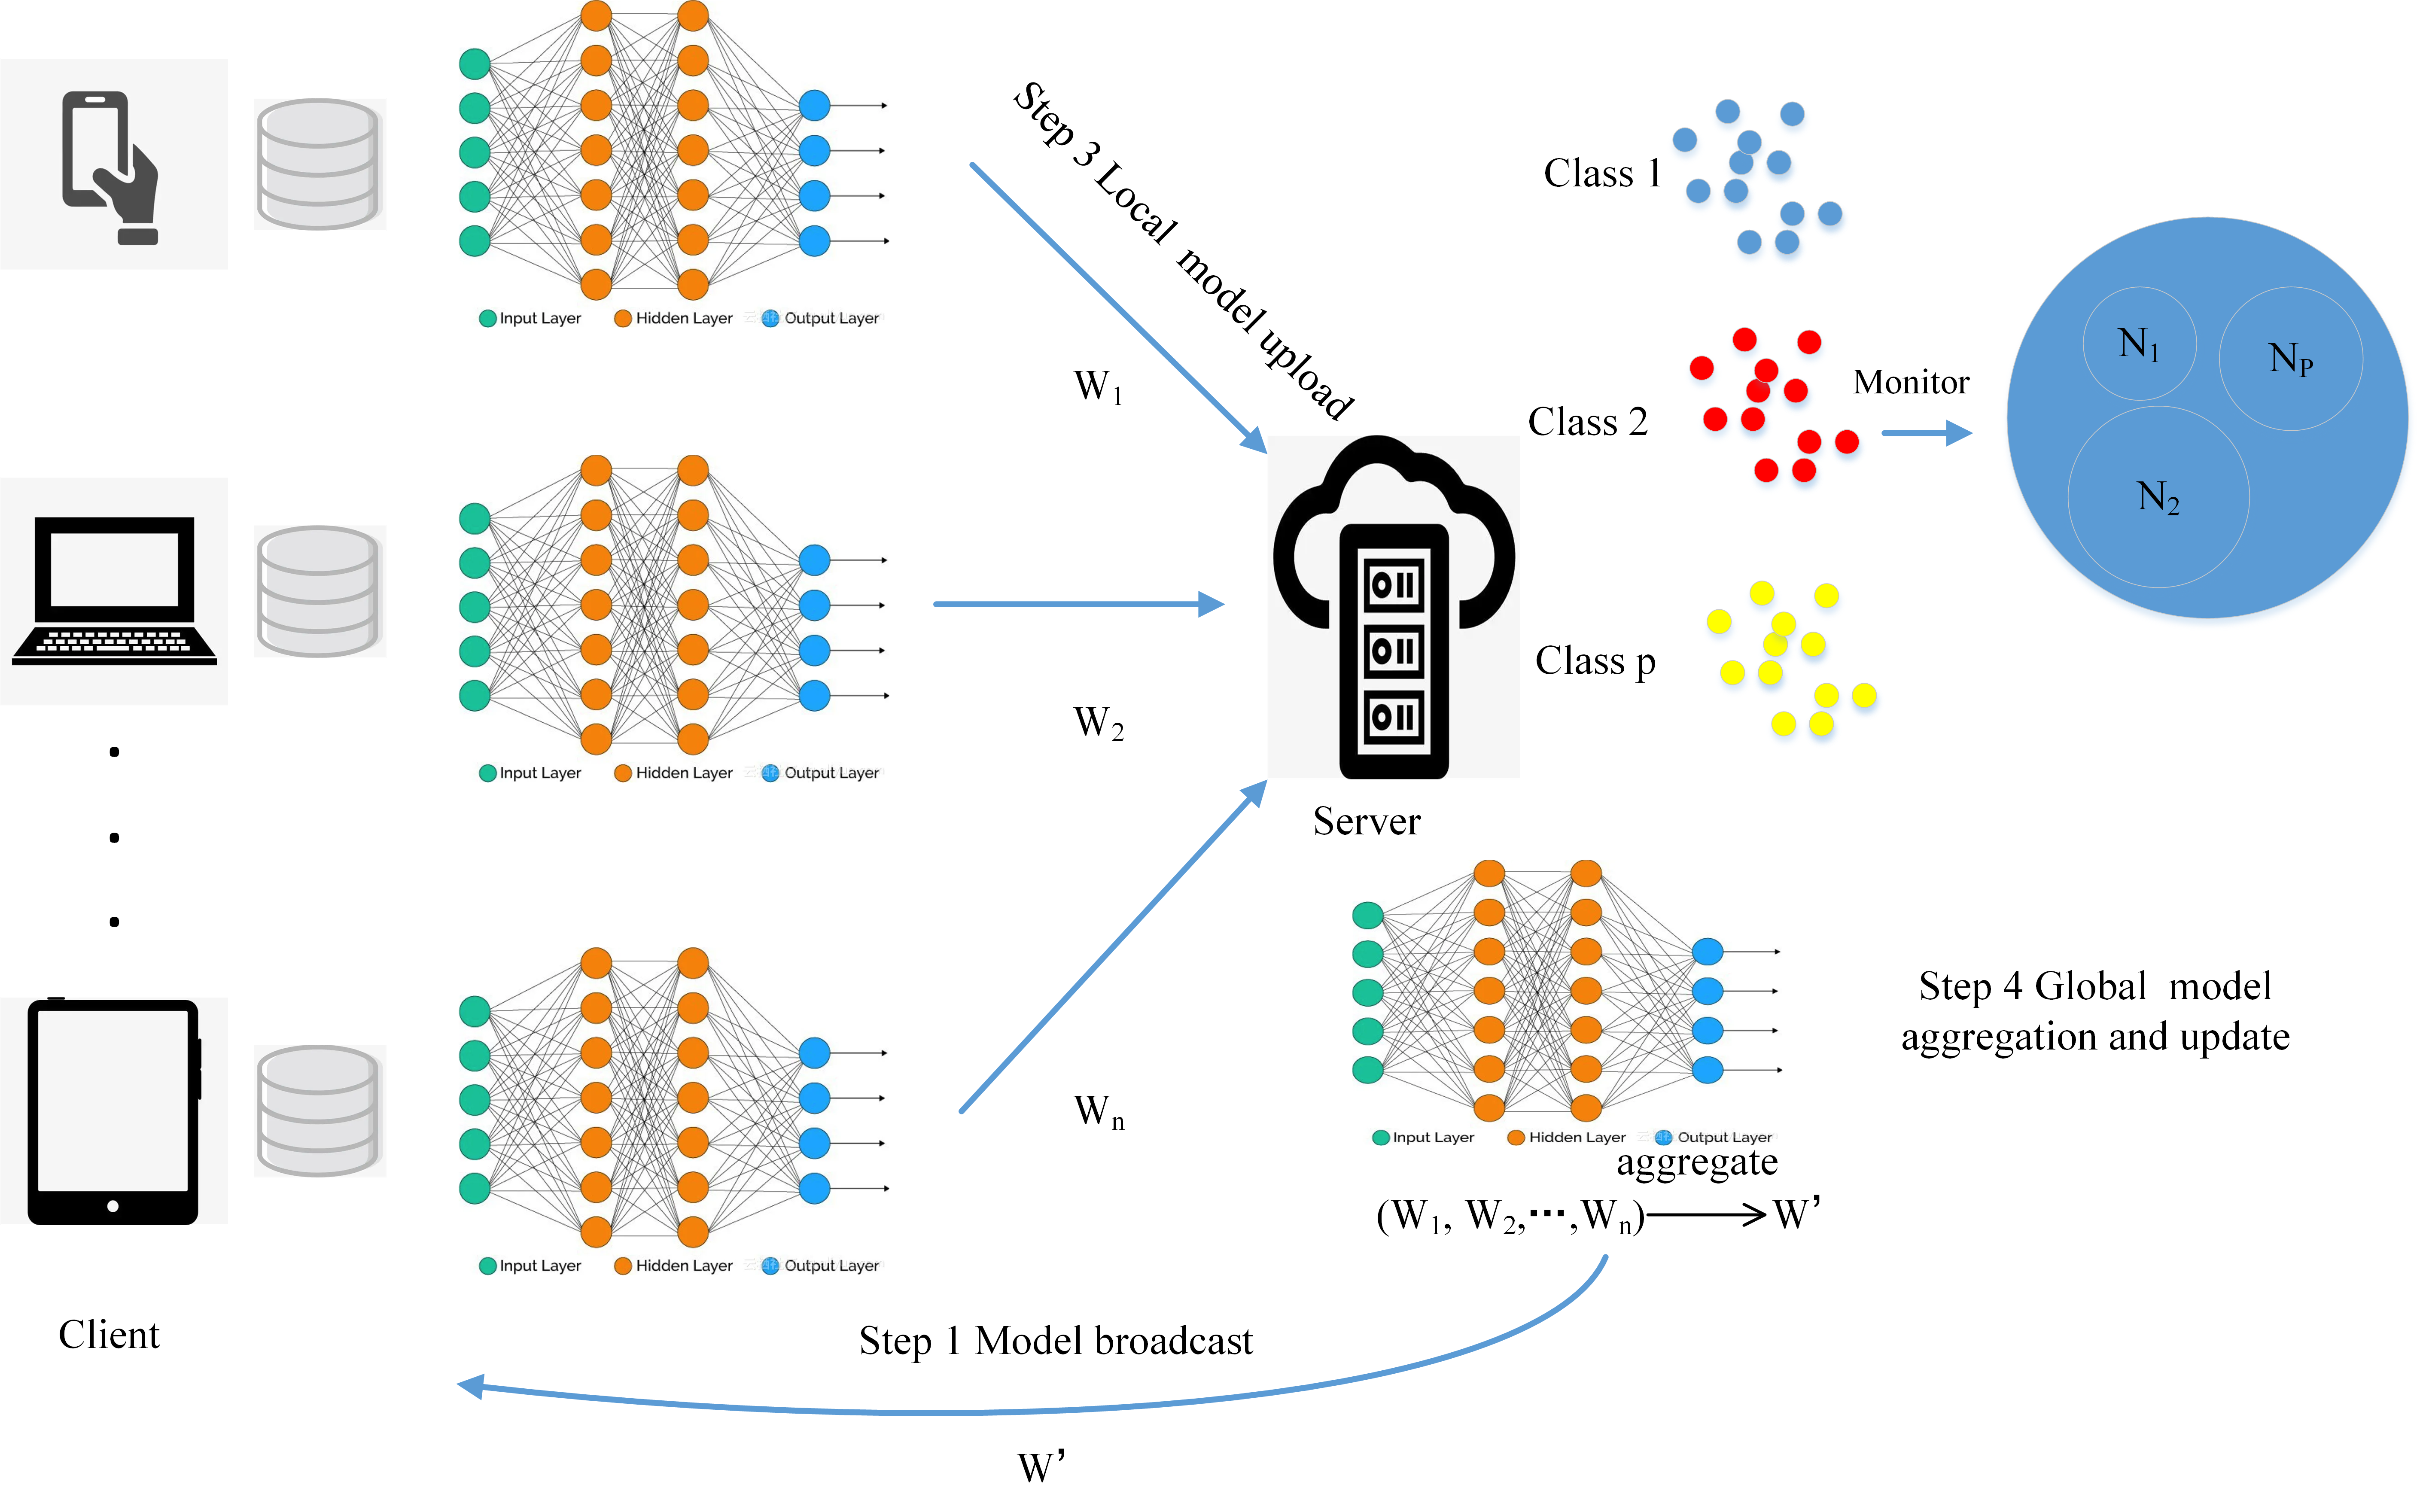
\includegraphics[scale=0.45]{estimation.png}
		\caption{Data distribution estimation based on model.}
		\label{Data distribution estimation}
	\end{figure*}
	
	\textbf{\DIFdelbegin \DIFdel{Gradient}\DIFdelend \DIFaddbegin \DIFadd{Gradient-based methods.}\DIFaddend } \DIFdelbegin \DIFdel{: }\DIFdelend Firstly, the relationship between the model's gradients and the sample numbers of different classes is analyzed. The model gradients are calculated on the class-balanced auxiliary datasets. And then the sample numbers of different classes can be estimated by the gradients.
	
	\DIFdelbegin \DIFdel{Wang et al. \mbox{%DIFAUXCMD
			\cite{wang2021addressing} }\hspace{0pt}%DIFAUXCMD
		analyze the sample quantity according to gradient magnitude. }\DIFdelend However, this method needs auxiliary data which may be not available under certain conditions.
	\DIFdelbegin \DIFdel{The server will feed samples of every class }\DIFdelend \DIFaddbegin 
	
	\DIFadd{Wang et al. \mbox{%DIFAUXCMD
			\cite{wang2021addressing} }\hspace{0pt}%DIFAUXCMD
		proposed a model for continuously monitoring the composition of training data when new data is constantly generated by client devices. It uses an auxiliary dataset that is balanced in class distribution. At time step $t+1$, the model downloads the global model $G_t$, feeds the samples }\DIFaddend in the auxiliary \DIFdelbegin \DIFdel{data singly to the global model. Then, according to weight updates corresponding to all classes, the server infers the global data distribution. This method needs all clients to upload the total sample numbers. Through experiments, the average }\DIFdelend \DIFaddbegin \DIFadd{dataset into $G_t$, and obtains the gradient updates w.r.t. the auxiliary dataset. By comparing these gradient updates with the global model $G_{t+1}$ at time step $t+1$, the model can infer the global class distribution. Experimental results }{\color{red} \DIFadd{on real-world datasets}} \DIFadd{show that the }\DIFaddend cosine similarity score between \DIFdelbegin \DIFdel{estimation and ground truth is above }\DIFdelend \DIFaddbegin \DIFadd{estimated and the ground-truth distribution achieves }\DIFaddend 0.98 \DIFaddbegin \DIFadd{on average}\DIFaddend . 
	
	Yang et al. \cite{yang2021federated} \DIFdelbegin \DIFdel{proposed an approach for detecting data distribution based on a balanced auxiliary dataset . The server can get the gradients vector brought by auxiliary data with regard to each class when the balanced auxiliary data instances are fed to the updated model. The distribution of the raw datacan be deduced from the gradient's expected results. 
		Additionally, each client's class imbalance degree is assessed using the Kullback-Leibler (KL) divergence. 
	}\DIFdelend \DIFaddbegin \DIFadd{revealed the correlation between gradients and class distributions: the expectations of gradient square of a trained model for different classes is approximately equal to the cardinality square of these classes. Based on this finding, they feed an auxiliary dataset into the trained global model to obtain the gradient updates for different classes. These gradient updates are then used to approximate the global class distribution of training data. 
	}\DIFaddend 
	
	Chen et al. \cite{chen2021novel} proposed a \DIFdelbegin \DIFdel{novel distribution estimation method. In clientclass distribution estimation, quantities of samples for all classes can be calculated by the expectations of gradients squared norms for all classes on local updated models. Then, the global class distribution is estimated by maximizing loss .
	}\DIFdelend \DIFaddbegin \DIFadd{method for class distribution estimation based on Yang et al.' finding \mbox{%DIFAUXCMD
			\cite{yang2021federated} }\hspace{0pt}%DIFAUXCMD
		about the correlation between gradients and class distributions. However, their method does not require auxiliary datasets. For each client, they compute the gradient updates of the client's trained model, from which they can directly derive the class distribution of the client's local dataset. The global distribution can then be formulated as the weighted average of all clients' class distributions, where the weights are set of parameters to be learned. Therefore, training the global model can be regarded as the process of minimizing the overall loss by quasi two-party theory }{\color{red}\DIFadd{add citation}}\DIFadd{. They propose an algorithm that optimizes the weights and model parameters alternatively for model training.  
	}\DIFaddend 
	
	\DIFdelbegin \DIFdel{For the purpose of reducing catastrophic forgetting from both }\DIFdelend \DIFaddbegin \DIFadd{Dong et al. \mbox{%DIFAUXCMD
			\cite{dong2022federated} }\hspace{0pt}%DIFAUXCMD
		assumed that the data imbalance in FL may vary over time on both the }\DIFaddend local and global \DIFdelbegin \DIFdel{perspectives, Dong et al. \mbox{%DIFAUXCMD
			\cite{dong2022federated} }\hspace{0pt}%DIFAUXCMD
		presented a Global-Local Forgetting Compensation model . }\DIFdelend \DIFaddbegin \DIFadd{level. Moreover, they assume that there could be new data for unseen classes appear in the dataset. As such, a local or global model may forget information about old classes due to limited storage. To handle such a catastrophic forgetting problem, they propose a global-local forgetting compensation model. }\DIFaddend In particular, local clients will \DIFdelbegin \DIFdel{use a }\DIFdelend \DIFaddbegin \DIFadd{address the forgetting problem through a class-aware gradient compensation loss and a class-semantic distillation loss. On the global level, the model saves a set of old global models. Once an unseen class is encountered, the model uses a }\DIFaddend prototype gradient-based communication mechanism to send perturbed prototype samples of \DIFdelbegin \DIFdel{newly discovered classes }\DIFdelend \DIFaddbegin \DIFadd{the new class }\DIFaddend to the proxy server\DIFdelbegin \DIFdel{when they have discovered them}\DIFdelend . The proxy server reconstructs the perturbed prototype samples after receiving these gradients\DIFaddbegin \DIFadd{, }\DIFaddend and uses them to track the effectiveness of \DIFdelbegin \DIFdel{these }\DIFdelend \DIFaddbegin \DIFadd{the saved }\DIFaddend old global models\DIFdelbegin \DIFdel{until the best one is discovered}\DIFdelend \DIFaddbegin \DIFadd{. The best performed old model will be used for relation distillation in order to tackle the global forgetting problem}\DIFaddend .
	
	\textbf{Loss}: \DIFdelbegin \DIFdel{In deep learning models, the loss function is used to evaluate the performance of the model in the training process . By analyzing the loss function in the FL environment, the classification performance on the client's local dataset can be analyzed. The subsequent training process can be adjusted by the value of }\DIFdelend \DIFaddbegin \DIFadd{Usually, }\DIFaddend loss \DIFdelbegin \DIFdel{function}\DIFdelend \DIFaddbegin \DIFadd{functions are used to guide the training process of deep learning models. The values of losses also reflect the performance of a model, i.e., higher loss indicates worse performance}\DIFaddend . There are studies that use techniques\DIFdelbegin \DIFdel{like }\DIFdelend \DIFaddbegin \DIFadd{, such as }\DIFaddend active learning and reinforcement learning\DIFdelbegin \DIFdel{to implicitly learn }\DIFdelend \DIFaddbegin \DIFadd{, to implicitly infer }\DIFaddend the data composition \DIFdelbegin \DIFdel{as the optimization condition}\DIFdelend \DIFaddbegin \DIFadd{for optimizing global model}\DIFaddend . 
	
	
	\DIFdelbegin \DIFdel{In the class imbalanced data , samples of }\DIFdelend \DIFaddbegin \DIFadd{For dataset with high data imbalance, }\DIFaddend the minority class \DIFdelbegin \DIFdel{will have significantly }\DIFdelend \DIFaddbegin \DIFadd{usually have much }\DIFaddend higher loss than \DIFdelbegin \DIFdel{majority class samples}\DIFdelend \DIFaddbegin \DIFadd{the majority class}\DIFaddend . In \cite{goetz2019active}, the value of loss function \DIFdelbegin \DIFdel{is used as a value function that reflects how useful the data on that clientis during each FL training round, therefore, there will be a greater selection likelihood of clients who have more }\DIFdelend \DIFaddbegin \DIFadd{of one client is considered to reflect the usefulness of the client's dataset during a training round. Therefore, the clients that are considered more useful (i.e., having more }\DIFaddend samples belong to the global minority class\DIFdelbegin \DIFdel{in order to solve }\DIFdelend \DIFaddbegin \DIFadd{) will be more likely to be selected in the subsequent training rounds in order to handle }\DIFaddend the issue of class imbalance. 
	
	Shen et al. \cite{shen2021agnostic} \DIFdelbegin \DIFdel{imposed constraints on }\DIFdelend \DIFaddbegin \DIFadd{added a constraint to }\DIFaddend the standard FL \DIFdelbegin \DIFdel{formulation so that }\DIFdelend \DIFaddbegin \DIFadd{scheme: }\DIFaddend the empirical loss \DIFdelbegin \DIFdel{on }\DIFdelend \DIFaddbegin \DIFadd{of }\DIFaddend every client should not overly exceed the average empirical loss. \DIFdelbegin \DIFdel{Such constraints are shown to force the }\DIFdelend \DIFaddbegin \DIFadd{Under the heterogeneous data configuration with mismatch imbalance, this constraint is shown to make the global }\DIFaddend classifier to account for all classes equally\DIFdelbegin \DIFdel{and hence }\DIFdelend \DIFaddbegin \DIFadd{, and hence, }\DIFaddend mitigate the detrimental effect of class imbalance\DIFdelbegin \DIFdel{, under a type of heterogeneous data configuration that captures the mismatch between the local and global imbalance. }\DIFdelend \DIFaddbegin \DIFadd{. }{\color{red} \DIFadd{Confirm this is correct.}} 
	\DIFaddend 
	
	\DIFdelbegin \DIFdel{A Global-Regularized Personalization (GRP-FED) technique was presented by }\DIFdelend Chou et al \cite{chou2022grp} \DIFaddbegin \DIFadd{proposed a global-regularized personalization (GRP-FED) technique for FL}\DIFaddend . They aim at \DIFdelbegin \DIFdel{fair classification performance for each client. If the standard deviation of the global training loss in all clients is high, the global training loss is quite different and the global model may suffer from client imbalance. }\DIFdelend \DIFaddbegin \DIFadd{improving the fairness among all clients in terms of their contributions to the global model. They propose an adaptive algorithm that adaptively adjust the weight of each client and aggregates a fair global model. }{\color{red} \DIFadd{Confirm this is correct.}}  
	\DIFaddend 
	
	\textbf{Performance of model}: The subsequent federated learning process is adjusted by the classification performance of the model on each class sample. The class with higher classification accuracy usually has a larger number of samples. This method cannot estimate the distribution information of the data, and can only guide the subsequent federated learning process through the classification performance of each class sample. For example, in client selection based methods for solving the calss imbalance problem, clients with better comprehensive classification performance are selected to participate in the training, so as to improve the performance of the global model.
	
	To alleviate the impact of \DIFdelbegin \DIFdel{label distribution skewness}\DIFdelend \DIFaddbegin \DIFadd{skewness in label distribution of clients' datasets}\DIFaddend , Mou et al. \cite{mou2021optimized} \DIFdelbegin \DIFdel{employ }\DIFdelend \DIFaddbegin \DIFadd{employed }\DIFaddend a balanced global validation dataset on the server side to score the performance of each client's model\DIFdelbegin \DIFdel{, which is a very straightforwardmethod to evaluate clients}\DIFdelend \DIFaddbegin \DIFadd{. This provides a straightforward, yet easy to operate method for client evaluation}\DIFaddend .
	
	Geng et al. \cite{geng2022bearing} \DIFdelbegin \DIFdel{presented the bearing fault diagnosis FL algorithm. Each client needs to upload its F1-score on local data. 
		The F1 value can reflect its overall classification performance. 
	}\DIFdelend \DIFaddbegin \DIFadd{proposed to weight local models based on their F$_1$ scores in the model aggregation process. As such, the aggregation policy in FL is enhanced by increasing the weight of high-quality client models. 
	}\DIFaddend 
	
	Hao et al. \cite{hao2021towards} proposed \DIFaddbegin \DIFadd{the }\DIFaddend zero-shot data generation (ZSDG) \DIFdelbegin \DIFdel{, }\DIFdelend \DIFaddbegin \DIFadd{algorithm, which can be used }\DIFaddend to generate labeled synthetic data for data-augmentation \DIFdelbegin \DIFdel{at the clients }\DIFdelend \DIFaddbegin \DIFadd{either at the client }\DIFaddend or the server side. ZSDG \DIFdelbegin \DIFdel{either utilizes the }\DIFdelend \DIFaddbegin \DIFadd{can be used in two ways, both of which can alleviate the data imbalance issue. First, ZSDG can utilize the }\DIFaddend pre-updated global model to generate synthetic data of the desired classes on the client side\DIFdelbegin \DIFdel{or utilizes }\DIFdelend \DIFaddbegin \DIFadd{. Second, it can utilize }\DIFaddend the post-updated local models to generate synthetic data of the desired classes on the server side without access to any non-local data. 
	
	\subsection{Cluster}
	\DIFdelbegin \DIFdel{These clustered FL methods often cluster clients into }\DIFdelend \DIFaddbegin \DIFadd{This group of methods clusters clients into different }\DIFaddend groups based on \DIFdelbegin \DIFdel{certain client uploaded information. These information are limited to }\DIFdelend \DIFaddbegin \DIFadd{the clients' certain attributes. In order to protect user privacy, the attributes disclosed by clients to the server should only be restricted to certain information such as }\DIFaddend model weights \cite{ghosh2019robust} \cite{xie2020multi}, gradients \cite{briggs2020federated} \cite{sattler2020clustered}, local optima \cite{ghosh2020efficient} \cite{mansour2020three}, etc. \DIFdelbegin \DIFdel{, as they must be gathered in federated settings without sharing local data. An intuitive solution to this issue is to cluster clients, then one personalized model is trained for each cluster \mbox{%DIFAUXCMD
			\cite{fu2021cic}}\hspace{0pt}%DIFAUXCMD
		, or choose clients based on these clusters to make the global dataset become class balanced. For example, as }\DIFdelend \DIFaddbegin \DIFadd{Based on the clustering results, the server can then use different strategies for different clusters in order to alleviate data balance issue. As }\DIFaddend shown in Fig. \ref{Client clusters}, all clients are grouped into 4 clusters according to the type of \DIFdelbegin \DIFdel{pictures }\DIFdelend \DIFaddbegin \DIFadd{images }\DIFaddend they store. \DIFdelbegin \DIFdel{These clusters can then be combined to solve the class imbalance in FL}\DIFdelend \DIFaddbegin \DIFadd{Then for each cluster, different strategies can be used}\DIFaddend , such as generating a personalized model for each cluster, \DIFdelbegin \DIFdel{sampling sample or client selectionaccording to clusters to achieve class balance in the global data , etc}\DIFdelend \DIFaddbegin \DIFadd{data sampling and client selection, which aim to address global data imbalance}\DIFaddend . 
	
	\begin{figure}[h]
		\centering
		\includegraphics[scale=0.35]{cluster.png}
		\caption{Client clusters.}
		\label{Client clusters}
	\end{figure}
	
	Zhao et al. \cite{zhao2020cluster} employed an agglomerative hierarchical clustering algorithm to cluster clients into groups. The \DIFdelbegin \DIFdel{input to the clustering model is }\DIFdelend \DIFaddbegin \DIFadd{features in clustering include }\DIFaddend the parameters of local models that are trained and uploaded by \DIFdelbegin \DIFdel{these }\DIFdelend clients. 
	
	Wang et al. \cite{wang2021adaptive} proposed a new weighted clustered FL (CFL) model based on adaptive clustering algorithm. At each round of FL training, clients are clustered into groups based on the cosine similarity of the uploaded local gradients. Each client not only uploads the local gradient but also uploads its class imbalance degree \DIFaddbegin \DIFadd{to the server}\DIFaddend .  
	
	Fu et al. \cite{fu2021cic} proposed a class imbalance-aware clustered FL method (CIC-FL). Every client \DIFdelbegin \DIFdel{calculates a feature }\DIFdelend \DIFaddbegin \DIFadd{computes a feature vector}\DIFaddend , using weight updates and the label-wise gradients of the global model and sends it to the server. CIC-FL employs a top-down hierarchical clustering process. Then, the server iteratively conducts bi-partitioning to partition these clients into two clusters. 
	
	\subsection{Bottom-up Class Distribution Estimation}
	\DIFdelbegin \DIFdel{Clients themselves judge }\DIFdelend \DIFaddbegin \DIFadd{Since clients have full access to their local models, they can infer }\DIFaddend the data distribution according to the state of the FL model, or \DIFdelbegin \DIFdel{judge }\DIFdelend \DIFaddbegin \DIFadd{infer }\DIFaddend the degree of similarity between the local data and the global data distribution.
	
	To protect clients' \DIFdelbegin \DIFdel{private}\DIFdelend \DIFaddbegin \DIFadd{privacy}\DIFaddend , Zhang et al. \cite{zhang2021fedsens} proposed a FedSens method, \DIFdelbegin \DIFdel{clients judge }\DIFdelend \DIFaddbegin \DIFadd{where clients decide }\DIFaddend whether to participate in this round of learning based on \DIFaddbegin \DIFadd{the }\DIFaddend current state, and \DIFaddbegin \DIFadd{the }\DIFaddend extrinsic-intrinsic reward. The current state \DIFaddbegin \DIFadd{that a client should consider }\DIFaddend is the classification performance on each class and the energy needed to train a local model at each device. \DIFaddbegin \DIFadd{The reward for each client depends on the client's dataset. }\DIFaddend If a client has \DIFdelbegin \DIFdel{class }\DIFdelend balanced local data, \DIFdelbegin \DIFdel{it }\DIFdelend \DIFaddbegin \DIFadd{the client }\DIFaddend should obtain a bigger reward.
	
	In Dubhe \cite{zhang2021dubhe}, each \DIFdelbegin \DIFdel{participant }\DIFdelend \DIFaddbegin \DIFadd{participating client }\DIFaddend calculates the local data distribution, and then uses the homomorphic encryption method to encrypt the \DIFdelbegin \DIFdel{data distributiondata}\DIFdelend \DIFaddbegin \DIFadd{distribution}\DIFaddend . The server adds the \DIFdelbegin \DIFdel{data distribution data of all users }\DIFdelend \DIFaddbegin \DIFadd{distributions of all clients }\DIFaddend according to additive homomorphism\DIFdelbegin \DIFdel{. After that, the server returns the calculation result to  users, and users }\DIFdelend \DIFaddbegin \DIFadd{, the result of which is then returned to all clients. The clients then }\DIFaddend decrypt the result to obtain the overall class distribution. 
	
	Li et al. \cite{li2021sample} proposed a data selection method for FL\DIFaddbegin \DIFadd{. Instead of exposing local data or distribution of local data}\DIFaddend , each client only reports 1-bit information, i.e., \DIFdelbegin \DIFdel{whether or not }\DIFdelend \DIFaddbegin \DIFadd{if }\DIFaddend the client's data is relevant \DIFdelbegin \DIFdel{, }\DIFdelend to the server \DIFaddbegin \DIFadd{or not}\DIFaddend . 
	
	Hahn et al. \cite{hahn2019privacy} proposed \DIFdelbegin \DIFdel{that the server estimates the posterior distributions of parameters of a parametrized probabilistic function for estimating an unknown arbitrary probability density, by exchanging information with local clients. The information is a similarity between generated samples , which are aimed to be close to perturbed samples}\DIFdelend \DIFaddbegin \DIFadd{an approximate Bayesian computation-based Gaussians Mixture Model called ``Federated ABCGMM'', which can oversample data in a minor class by estimating the posterior distribution of model parameters. The algorithm selects candidate parameters from the posterior distribution, and generate samples based on the selected parameters. These samples generated by the central server are then shared to clients, who will compute the similarity between these samples and their local samples. Based on the resulted similarities amongst all clients, the sampled parameter candidate will be determined to be accepted or rejected at the CS. When the process is iterated, the accepted set of parameters becomes close to its true posterior distribution}\DIFaddend .
	
	These class estimation methods are listed in Table \ref{class imbalance estimation methods}.
	
	\begin{table*}[!t]
		\centering
		\caption{Representatives of reviewed class imbalance estimation methods in FL}	  
		\label{class imbalance estimation methods}     		       	
		\begin{tabular}{cp{6.5cm}p{6.5cm}}
			\hline
			Strategy & Representative articles& Detailed description \\ 
			\hline
			Updating distribution information& Mhaisen et al. \cite{mhaisen2021optimal}
			Geng et al. \cite{geng2022bearing}
			Mrad et al. \cite{mrad2021federated}
			Duan et al. \cite{duan2019astraea} \cite{duan2020self}& The server collects uploaded data distribution information, clients' privacy will be leaked to some extent.  \\ \hline
			Loss function& Shen et al. \cite{shen2021agnostic} Goetz et al. \cite{goetz2019active} Chou et al. \cite{chou2022grp}&The server estimates the class distribution according to the value of loss function\\  \hline
			Gradient& Chen et al. \cite{chen2021novel} Hao et al. \cite{hao2021towards} Wang et al. \cite{wang2021addressing} Yang et al. \cite{yang2021federated}&The server estimates the class distribution according to gradients\\ \hline
			Model performance& Mou et al. \cite{mou2021optimized}&The server estimates the class distribution according to model performance \\ \hline
			Clustering algorithm& Fu et al.\cite{fu2021cic} Zhao et al. \cite{zhao2020cluster} Wang et al. \cite{wang2021adaptive} & Clients are clustered into clusters, the server solves the class imbalance problem according to these clusters\\  	\hline	
			Bottom-up method&  Zhang et al. \cite{zhang2021fedsens} Zhang et al. \cite{zhang2021dubhe} Li et al. \cite{li2021sample}  Hahn et al. \cite{hahn2019privacy}&Clients estimate class distribution according to class distribution information obtained by typical protocol or model performance\\  		
			\hline
		\end{tabular}
		
	\end{table*}
	
	\subsection{Class Estimation On Client Or Server Side}
	\DIFdelbegin \DIFdel{In this section, we divide these class distribution estimation methods }\DIFdelend \DIFaddbegin \DIFadd{We divide all the methods for estimating class distribution }\DIFaddend in FL into two \DIFdelbegin \DIFdel{groups: class imbalance estimation on the client sideand class imbalance estimation on the server side. These methods are summarized in Table3. 
	}\DIFdelend \DIFaddbegin \DIFadd{types: (1) estimation conducted on the server side; and (2) estimation conducted on client side. We summarize this categorization in Table~\ref{tab:class_estimation_server_or_client}. 
	}\DIFaddend 
	
	Most of the methods for data distribution estimation on the server side are to solve the global imbalance problem. The data distribution exploration methods mentioned in the previous section, except for the bottom-up method, all belong to the data distribution evaluation on the server side.
	
	\begin{table*}[htbp]
		\centering
		\caption{Representatives of reviewed class imbalance estimation methods in FL}	       		       	
		\begin{tabular}{cp{8.2cm}p{7.8cm}}
			\hline
			Strategy & Representative articles& Detailed description \\ 
			\hline
			Server side&Mhaisen et al. \cite{mhaisen2021optimal}
			Geng et al. \cite{geng2022bearing}
			Mrad et al. \cite{mrad2021federated}
			Duan et al. \cite{duan2019astraea} \cite{duan2020self} 
			Chen et al. \cite{chen2021novel}
			Hahn et al. \cite{hahn2019privacy}
			Chou et al. \cite{chou2022grp} 
			Hao et al. \cite{hao2021towards} 
			Wang et al. \cite{wang2021addressing} 
			Yang et al. \cite{yang2021federated}
			Mou et al. \cite{mou2021optimized}
			Fu et al.\cite{fu2021cic} 
			Zhao et al. \cite{zhao2020cluster} 
			Wang et al. \cite{wang2021adaptive} 
			Shen et al. \cite{shen2021agnostic}
			Goetz et al. \cite{goetz2019active}
			&The server evaluates the class distribution of the global data through the class distribution of each client, local models, or model performance\\ \hline
			Client side &	Zhang et al. \cite{zhang2021fedsens} 
			Zhang et al. \cite{zhang2021dubhe} 
			Li et al. \cite{li2021sample} &	Clients calculate the global class distribution either by model performance or by a specific protocol\\			 				
			\hline
			\DIFaddbeginFL \label{tab:class_estimation_server_or_client}
			\DIFaddendFL \end{tabular}
	\end{table*}
	
	\section{Class Imbalanced Data Classification Approaches In Federated Learning}
	There is an extensive investigation into class imbalance in traditional machine learning \cite{guo2008class} \cite{ali2013classification}. The impact of class imbalance depends on the imbalance level, concept complexity, and size of training data \cite{japkowicz2002class}. The main reasons for the class imbalance that degrades performance include information gaps brought by limited sample sizes, class overlap, and small disjuncts within a class \cite{ali2013classification}. Traditional methods to address the class imbalance problem in machine learning can be divided into five categories: preprocessing methods, cost-sensitive learning, algorithm-centered methods, ensemble learning, and hybrid methods \cite{liu2008exploratory} \cite{xiao2021experimental}.
	
	\begin{figure*}[!t]
		\centering
		\includegraphics[scale=0.6]{methods.jpg}
		\caption{Approaches for imbalance data.}
		\label{Approaches for imbalance data}
	\end{figure*}
	
	In addition to the above-mentioned methods used in traditional machine learning, based on the characteristics of FL, there are also technologies based on aggregation technology and user personalization. So far, there is no research on the combination of ensemble learning and FL for solving the class imbalance problem. Next, as shown in Fig. \ref{Approaches for imbalance data}, we will divide these methods of solving the class imbalance problem in FL into three category: sampling method, algorithm-center method, and system method. Sampling method is a kind of preprocessing technique, it processes the training data, so that the class distribution of training data is balanced. Algorithm-center method needs to change the classification algorithm, mainly including changing the loss function and modifying the algorithm itself or input, making the algorithm more sensitive to minority classes. System method mainly includes aggregation-based method, personalization method, system modification method, and meta-learning method. 
	
	\subsection{Sampling Techniques}
	By sampling samples or clients, class balance can be achieved to improve the classification performance. Sampling is a popular option for researchers who are not machine learning professionals. It is much simpler to directly use in both single and ensemble models.
	
	Client side sample sampling(local imbalance): The label sampling probabilities are made more similar across clients by data resampling. The deviation of the participated class proportion from the global class proportion, causing classification performance degradation. The variance in participated class proportion will cause fluctuation in training process \cite{duan2019astraea}. Sampling methods make the convergence of FL model faster. The local data of each client has reached the class balance, but the global balance of the overall dataset cannot be guaranteed.
	
	Server side sample sampling or client sampling(global imbalance): To solve the global imbalance problem, it is important to estimate data distribution of the global dataset. Therefore, this method is more complex than client side data sampling. 
	
	Data sampling may result in classification performance decreasing on a client \cite{tangdata}. It could make the models over-fitting on the minority classes or under-fitting on the majority classes \cite{cao2019learning}. One explanation for the phenomena could be that the imbalanced data resampling hurts individual clients' learning of "Special Knowledge" (local dataset) in the FL model, leading to low final accuracy \cite{cao2019learning}. 
	
	In this section, we will introduce three kinds of sampling technologies in FL: sample sampling, client sampling, and hybridization of sample sampling and client sampling.
	\subsubsection{Sample Sampling}
	Sampling is a data preprocessing technique that processes data before model training to improve model performance.
	Sampling strategies are used to rebalance the sample space for a class imbalanced dataset, in order to alleviate the effect of the class imbalanced distribution on the learning process in machine learning. Sampling strategies are more adaptable because they are unrelated to a specific classifier \cite{lopez2013insight}. These strategies can be categorized into three groups based on the method used to balance the distribution of these classes in a dataset \cite{haixiang2017learning}:
	
	\begin{figure}[h]
		\centering 
		\subfloat[Oversampling method.]{\includegraphics[scale=0.75]{oversampling.png}
			\label{fig_first_case}}
		\hfil
		\subfloat[Undersampling method.]{\includegraphics[scale=0.75]{undersampling.png}
			\label{fig_first_case}}
		\caption{Sampling methods.}
		\label{Sampling methods}
	\end{figure}
	
	\begin{itemize}
		\item  Over-sampling methods: producing new minority class samples, as shown in Fig. \ref{Sampling methods} (a). SMOTE \cite{chawla2002smote} and randomly duplicating the minority samples are two techniques that are frequently used to produce synthetic minority samples. 
		
		\item Under-sampling methods: removing the inherent samples in the majority class, as shown in Fig. \ref{Sampling methods} (b). The most straightforward yet efficient technique is Random Under Sampling (RUS) \cite{tahir2009multiple}, which involves randomly removing examples from the majority class.
		
		\item  Hybrid methods: these methods are a combination of the over-sampling method and the under-sampling method.
	\end{itemize}
	
	In client-side sample sampling, since the amount of data in each client is usually small, over-sampling is usually employed. The most common and dominant technique to improve the performance of FL both globally and locally is local fine-tuning. A well-performed local update can significantly generate a better global model \cite{ran2021dynamic}. In server-side sample sampling, the server can choose the sampling method according to characteristics such as the size of dataset.
	
	Shingi et al. \cite{shingi2020federated} employed SMOTE method to oversample minority class data at the client level. 
	
	Hao et al. \cite{hao2021towards} proposed a novel zero-shot data generation (ZSDG) oversampling method to mitigate class imbalance in the FL system. They study two variants of this scheme, FL with ZSDG at the clients and FL with ZSDG at the server. Moreover, ZSDG encourages more uniform accuracy performance(fairness) across clients in federated networks. 
	
	Tijani et al. \cite{tijani2021federated} proposed a straightforward data extension method to deal with the severe label skew issue. Based on the classes that are missing from the client's private data, each client chooses a few extension samples from external data samples.
	
	Weinger et al. \cite{weinger2022enhancing} examined the impact of data over-sampling on IoT anomaly detection performance in FL. They use a set of over-sampling techniques including random oversampling, SMOTE \cite{chawla2002smote}, and a variant of SMOTE known as ADASYN \cite{he2008adaptive}. They aim to improve the quality of the client's local model, ensuring that these clients can contribute meaningful updates to the global model. Thus, they over-sample data locally on the client side.  local imbalance.
	
	Tang et al. \cite{tangdata} proposed an Imbalanced Weight Decay Sampling (IWDS) method, which is a simple but effective data resampling strategy. It dynamically regulates the sampling probability of different labels, remarkably accelerating the training process. In IWDS, the sampling weights of all data samples decay along the training round. Thus, to converge faster at the early training stage, it can make all clients have more similar label sampling probability. To better learn their special knowledge at the later stage, it can make all clients with the original label sampling probability. It is a kind of local sampling method.
	
	To oversample data in a minority class, Hahn et al. \cite{hahn2019privacy} presented an approximate bayesian computation-based gaussians mixture model that can estimate the posterior distribution of model parameters across institutions while maintaining anonymity. At the server, plausible perturbed samples in the minority class can be created, and when these samples are transmitted to the local client, they can improve the classification accuracy for the imbalanced data.
	
	\subsubsection{Client Sampling}
	There are two major reasons to sample clients instead of selecting all clients to participate in each iteration of FL. One is that not all clients are always accessible. For instance, some clients may not have enough power or may be turned off when the server is polling. The fact that not all clients have access to data distributions that are comparable to the underlying global data distributions is another factor. The learning process would converge slowly or even diverge due to the lack of similarity between the distributions of specific clients and the global distribution \cite{chen2021novel} \cite{goetz2019active}. 
	
	Random client selection aggravates the biased client participation when data among clients are non-IID and the global data distribution is biased \cite{zhang2021dubhe}. Many methods select a client set with minimal class imbalance. This will result in less diversity in generated local models. This also leads to the generated global model with poor robustness. 
	
	\begin{figure}[h]
		\centering
		\includegraphics[scale=0.45]{client sampling.png}
		\caption{Client sampling.}
		\label{Client sampling}
	\end{figure}
	
	As shown in Fig. \ref{Client sampling}, client sampling method is mainly applied to energy-constrained FL models, for example unmanned aerial vehicles(UAV) networks and mobile devices. Client sampling can combine with optimization method, ranking method, clustering method, and bottom-up method. 
	
	Optimization-based client sampling method selects a class balanced client set under the condition of optimization of some constraints, such as communication cost. 
	
	Mrad et al. \cite{mrad2021federated} proposed a solution to the problem of class imbalance in FL for energy-constrained unmanned aerial vehicles(UAV) networks while considering the limited availability of UAVs due to their stringent energy constraints. Their aim is to obtain a reliable and stable performance of FL for UAVs network, while considering the class imbalance problem. The optimization problem is to select the set of UAVs that delivers the lowest class imbalance, to improve classification accuracy.
	
	In order to reduce the distribution distance between edge devices, Mhaisen et al. \cite{mhaisen2021optimal} developed an optimization problem that assigns edge nodes within their communication range. The formulated issue is transformed into an NP-Hard issue. They then suggested two solutions to this issue. The first is a branch and bound-based solution to a simplified linear version of the problem that assumes equal assignments between edges. The second strategy uses heuristics to greedily try to balance out class distributions among edge devices. 
	
	Yang et al. \cite{yang2021federated} employed combinatorial multi-Armed bandit (CMAB)\cite{chen2013combinatorial} to design a client set selection method based on a composition vector. This method can select a client set with minimal class imbalance. 
	
	Clients can be evaluated and ranked by indicators such as local data distribution and local model classification performance, and the top clients can be selected.
	
	For the class imbalanced FL, Chen et al. \cite{chen2021novel} presented a novel client sampling technique. One metric called client reward is used to assess which clients should be sampled. The client rewards are associated with cosine-based similarity between client and global distributions. A ranking of these clients can be determined by the rewards, and the top clients would then be sampled to participate in model updating.  
	
	In \cite{goetz2019active}, an active FL model is proposed. The benefit of training on various clients may differ significantly because the data on each client is highly variable. In order to enhance efficiency, clients are selected in each round of FL with a probability conditioned on the current model and the client data.
	
	In the cluster-based client sampling, clients are selected based on client clusters to ensure the class balance of the global dataset.
	
	Zhao et al. \cite{zhao2020cluster} proposed a cluster-based solution to improve the accuracy of the minority class at the low expense of performance degradation on the majority class. Firstly, it performs FedAvg. Then, when the model is nearly stable, it clusters clients into groups using the hierarchical clustering method. Finally, participants are selected from these clusters for this round of training.
	
	In the bottom-up FL model, clients judge whether to participate in this round of training according to the data distribution of the global dataset or the performance of the current global model.
	
	In Dubhe \cite{zhang2021dubhe}, the data distribution information of each client is encoded using homomorphic encryption. The server adds the encrypted distribution information and then returns it back to clients. Each client calculates a participation probability according to the class distribution. They also propose a multi-time client selection method to further balance the global dataset in each training round. 
	
	Zhang et al. \cite{zhang2021fedsens} proposed a bottom-up device selection method to solve the class imbalance problem in abnormal health detection applications. To protect client's private, they judge whether to participate in this round of learning based on current state (the classification performance on each class and the energy needed to train a local model at each device) and extrinsic-intrinsic reward. The extrinsic reward is a feedback provided by current environment, it is defined as the global model's performance. The intrinsic reward considers the significance of the local model update and the energy cost of the device. 
	
	\subsubsection{Hybridization Of Sample Sampling And Client Sampling}
	The combination of sample sampling and client sampling can obtain more performance improvement than using only one of these two methods. Client selection is often combined with global data sampling to solve the global imbalance problem in FL. 
	
	Duan et al. \cite{duan2019astraea}\cite{duan2020self} proposed a self-balancing FL framework named Astraea. In \cite{duan2019astraea}, they employ data augmentation (over-sampling) method, to solve the global imbalance problem. In \cite{duan2020self}, it firstly performs both the z-score-based data augmentation and the under-sampling to solve the global imbalance of training data, according to distribution information from clients. Then, it uses a mediator which asynchronously receives and applies these updated models from participated clients to average the local imbalance. Therefore, the mediator can obtain a more balanced model by rescheduling clients' training. 
	
	Li et al. \cite{li2021sample} presented a productive hierarchical sample selection system that first chooses the best clients, and then their top-notch samples. Before training, they select clients relevant to the target FL task using a private set intersection based approach. Using a determinantal point process based method, they maximize both statistical homogeneity and content diversity of these chosen clients within one budget. Then, a selection strategy based on erroneous-aware importance is proposed to dynamically choose significant clients and samples during each iteration in FL training process. 
	
	\subsection{Algorithm-Centered Techniques}
	Algorithm-center method needs to change the classification algorithm, mainly including changing the loss function and modifying the algorithm itself, making the algorithm more sensitive to minority classes.
	
	\subsubsection{Cost-Sensitive Learning}
	Cost-sensitive assigns higher misclassification costs for minority class samples than for majority class samples. It is more computationally effective than resampling techniques, making it potentially more appropriate for massive data streams. However, compared to resampling techniques, it is much less popular. There are two possible reasons \cite{krawczyk2014cost}, one is that it is challenging to determine cost values. Most of the time, an expert cannot estimate the cost of misclassification because it cannot be determined from the data. Another reason is that cost-sensitive learning often needs to modify learning algorithms \cite{haixiang2017learning}. Therefore, it is necessary for users of FL model to have a comprehensive understanding of the classification algorithm.
	
	All algorithms in machine learning need to maximize or minimize a function, which is called the ``objective function''. Among them, a type of objective function that needs to be minimized is generally called ``loss function''. It can measure the predictive ability of the model based on the prediction results. The loss function is used to measure the inconsistency between the predicted value of the model and the real value. It is a non-negative real-valued function. The smaller the loss function, the better the performance of the model. By assigning higher misclassification costs for minority class samples than for majority class samples, the algorithm is more sensitive to the minority class. 
	
	Lin et al. \cite{lin2017focal} introduce the focal loss starting from the cross entropy (CE) loss for binary classification:
	\begin{subequations}\label{eqn-3}
		\begin{numcases}{CE(p,y)=}
		-log(p)& \text{ if } y=1 \label{eqn-3-1}\\
		1-log(p)& \text{ if } otherwise \label{eqn-3-1}
		\end{numcases}
	\end{subequations}
	In the above $y \in  \left\lbrace \pm 1 \right\rbrace  $ specifies the ground-truth class and $ p \in [0,1] $ is the model’s estimated probability for the class with label $ y = 1 $. For notational convenience, we define $ p_{t} $:
	\begin{subequations}\label{eqn-4}
		\begin{numcases}{p_{t}}
		p& \text{ if } y=1 \label{eqn-4-1}\\
		1-p& \text{ if } otherwise \label{eqn-4-1}
		\end{numcases}
	\end{subequations}
	and rewrite $ CE(p,y) = CE(p_{t}) = -log(p_{t}) $.
	
	Instead, the loss function is reshaped to down-weight easy positive samples(majority class samples) and thus concentrate training on difficult negative samples(minority class samples). Moreover, a modulating factor $ (1 - pt) ^{\gamma}  $ is added to the cross entropy loss, with tunable focusing parameter $  \gamma \ge 0 $.The focal loss is defined as:
	\begin{equation}
	Focal\_Loss(p_{t})= -(1 - pt) ^{\gamma} log(p_{t})
	\end{equation}
	
	There are two properties of the $ Focal\_Loss $:(1) The modulating factor is close to 1 and the loss is unchanged when the value of $ p_{t} $  is small and the sample is misclassified. The factor decreases to 0 and the loss for correctly classified sample is down-weighted as  $ p_{t} \to  1 $; (2) The rate at which easy classified samples are down-weighted is smoothly adjusted by the focusing parameter $ \gamma $. The $ Focal\_Loss $ is equal to $ CE $ for $ \gamma =0 $, and when $gamma$ increases, the modulating factor's influence also increases (we found $ \gamma =2 $ to work best in our experiments).
	
	Wang et al. \cite{wang2021addressing} proposed a monitoring scheme that can infer the distribution of global training data for each FL round according to gradients. They design a new Ratio Loss to mitigate the impact of the imbalance. Once the monitor detects a similar imbalanced distribution continuously, it will acknowledge clients apply a mitigation strategy that is based on the Ratio Loss function. 
	
	Sarkar et al. \cite{sarkar2020fed} proposed a new loss function called Fed-Focal Loss. It reshapes cross-entropy loss during training. According to the client's training performance, it down-weights the loss assigned to well-classified examples and focuses on hard-classified examples. Moreover, by leveraging a tunable sampling framework, the server selects the best-performing clients for global training. Therefore, this method improves the robustness of the global model. 
	
	Wang et al. \cite{wang2021federated} introduced a modified CE loss function denoted as balanced cross entropy (BCE) loss function. Moreover, they define a structural loss function, which is applied for preventing overfitting, and BN and dropout are the common methods. 
	
	
	Shen et al. \cite{shen2021agnostic} impose constraints on the standard FL formulation so that the empirical loss on every client should not overly exceed the average empirical loss. Such constraints are shown to force the classifier to account for all classes equally and hence mitigate the detrimental effect of class imbalance, under a type of heterogeneous data configuration that captures the mismatch between the local and global imbalance. their formulation can significantly improve the testing accuracy of the minority class, without compromising the overall performance.
	
	A novel Global-Local Forgetting Compensation model was created by Dong et al. \cite{dong2022federated}. It mainly comprises of a class-aware gradient compensation loss and a class-semantic relation distillation loss to battle local catastrophic forgetting induced by the class imbalance on the client side and global catastrophic forgetting caused by non-i.i.d. class imbalance across clients. While using the old global model with the best performance, a prototype gradient-based communication mechanism is created between the proxy server and clients for their private communication.
	
	\subsubsection{Algorithmic Classifier Modification}
	Most of algorighm-centered methods directly modify the learning process to raise the classifier's sensitivity to minority classes \cite{khan2017cost}. As shown in Fig. \ref{algorithm}, the modified model encourages clients to have a large margin for
	minority class.  
	
	\begin{figure}[h]
		\centering
		\includegraphics[scale=0.5]{algorithm.png}
		\centering
		\caption{Algorithm-centered approach.}
		\label{algorithm}
	\end{figure}
	
	Ran et al. \cite{ran2021dynamic} presented a Dynamic Margin for FL, which encourages each participant client to have a large margin for minority classes by adding a dynamic term into margins. Accordingly, in the local training phase, the original softmax is replaced with the dynamic margin softmax. Moreover, the cross-entropy loss is combined with dynamic margin.
	
	Hua et al. \cite{hua2020blockchain} improved the traditional SVM model by giving the majority and minority classes separate penalty components. This technique is capable of handling data with imbalanced traction and braking. 
	
	Federated fuzzy learning approach with class imbalanced data was proposed by Dust et al. \cite{dust2021federated}. They presented an imbalance adaption mechanism to increase the impacts of minority class samples in the fuzzy learning process in order to address the problem of class imbalance. By allowing the competent rules of the minority class to coexist with those of the majority class, this has the effect of preventing the model from being biased against the majority class. The main idea is to virtually oversample the minority class samples. 
	
	%algorithm +aggregation: 
	Li et al. proposed  \cite{li2021fedrs} a FedRS method. During local procedures, they advocate that the update of missing classes’ proxies should be restricted, thus, a restricted softmax is proposed. Adding "scaling factors" to the softmax operation is a simple method to put this into practice. Then, a fine-grained aggregation is based on $p_{k,c}=\frac{N_{k,c}}{ {\textstyle \sum_{k}^{}} N_{k,c}}$, where $N_{k,c}$ is the number of $ c $-th class samples on $ k $-th client. 
	
	\subsection{System-Centered Techniques}
	System method is to change the FL structure, it mainly includes aggregation-based method,  personalization method, and system modification method.
	\subsubsection{Aggregation Method}
	In the model aggregation stage, the weight of the local model requires a uniform evaluation standard. The only factor affecting the standard FedAvg algorithm, which uses class balanced samples, is the variation in data volume between clients. To improve the training of class imbalanced data sets, local models are weighted in model aggregation based on weight which may reflect the classification performance of local models \cite{geng2022bearing}. 
	
	Wang et al. \cite{wang2021adaptive} proposed a new weighted clustered FL (CFL) model based on an adaptive clustering algorithm. Then weighted per-cluster model aggregation is performed on the server side. Each cluster has a different weight to balance the contribution of each class of global training data. In addition, the weight of each cluster is optimized through the convergence rate analysis. 
	
	Geng et al. \cite{geng2022bearing} proposed a weighted aggregation policy based on F1-scores. In FL model aggregation, local models of clients are weighted based on the weighted F1-scores to improve performance based on class imbalanced data sets. They also proposed an improved aggregation algorithm that is based on the accuracy difference between client temporary accuracy and one base accuracy. This method can improve the accuracy of model aggregation and reduce communication time. %Bearing fault diagnosis based on improved FL algorithm
	
	Mou et al.  \cite{mou2021optimized} proposed to generate a global balanced dataset on the server side. Then a validation score $ s_{i} $ is calculated by evaluating the performance of the local model of client $ i $ on the balanced global dataset. Finally, each client aggregation weight is calculated based on the validation score. Different metrics such as accuracy, IoU, and cross-entropy loss are tried as the validation score. 
	
	\subsubsection{Personalization Method}
	Instead of learning a single global model for all clients, personalized models are trained for different clients or for each client cluster \cite{kairouz2021advances}.  This approach can be combined with the above-mentioned methods for solving the class imbalance problem.
	
	\begin{figure*}[h]
		\centering
		\includegraphics[scale=0.5]{personality.png}
		\caption{An illustration of personalization FL.}
		\label{personalization}
	\end{figure*}
	
	All clients are treated equally by the traditional FedAvg method, which ignores the different data distributions among clients and results in poor performance on the global model. Furthermore, major clients can easily dominate the FedAvg model, while the other clients are given up, where the classification performance drops drastically on them. Even if encouraging these worse clients to focus on global fairness \cite{mohri2019agnostic} \cite{li2019fair}, the performance gap between global and local tests is still significant \cite{jiang2019improving}, indicating that personalization is essential in the FL model \cite{chou2022grp}. In the personalization FL model, local clients train part of local models only on their local data \cite{fallah2020personalized} \cite{khodak2019adaptive} \cite{liang2020think}. As shown in Fig. \ref{personalization}, for each client cluster or each client, a personalized local model is generated based on the global model and its local data.
	
	Fu et al. \cite{fu2021cic} proposed a CIC-FL method for solving class imbalance issue in FL. Each client uses over-sample or under-sample to generate a balanced local dataset. Then they are clustered into groups. To address the class imbalance and data shift problem, one personalized model is trained in each cluster. 
	
	Chou et al. \cite{chou2022grp} presented a Global-Regularized Personalization (GRP-FED) method into FL, to address the problem of class imbalance by taking into account a single global model and personalized local models for different clients. The global model mitigates the problem of the global long-tailedness and treats clients fairly by using adaptive aggregation. Each client's local model is learned from the local data and aligns with its distribution for personalization. GRP-FED uses an adversarial discriminator to regularize the learned global-local features, preventing the local model from simply overfitting. 
	
	To process the contextual access abstraction for IoT devices,Yu et al. \cite{yu2020learning} designed a customized data augmentation approach. They design two mechanisms to address unbalanced records: context random sampling and adding contextual noise. The goal is to reduce the the correlation between environment variables/device states and IoT access with a certain action by performing random sampling on the environment variables and device states. Noise is added to the environment variables of the attack sample.
	
	Chen et al.\cite{chen2022personalized} designed a Deputy-Enhanced Transfer to smoothly transfer global knowledge to clients' personalized local models. They propose a Conjoint Prototype-Aligned (CPA) loss to address the class imbalance problem and make the FL framework's balanced optimization easier. The CPA loss calculates the global conjoint objective based on global imbalance and then adjusts the client-side local training through the prototype-aligned refinement to eliminate the imbalance gap with such a balanced goal, taking into account the inaccessibility of clients' local data to other clients and the server in the FL model.
	
	\subsubsection{System Modification Method}
	In addition to changing the classification algorithm, the structure of FL can also be changed to solve the class imbalance problem.
	
	Convolutional neural networks (CNNs) are used on both the client and server sides by Cheng et al. \cite{cheng2022blockchain} to extract practical features. The imbalanced input data causes the neural network to extract unbalanced features, so they first get a cluster for each class, which is then used to build the classifier. Then, using the categorical cross-entropy function as a guide, each client model is trained. With the help of blockchain technique, the traditional FL is enhanced without having to worry about the failure of the server and boosts the privacy of clients.
	
	Cheng et al. \cite{cheng2022class} proposed a class-imbalanced heterogeneous FL method. They use a convolutional neural network (CNN) on both the client and server sides to extract useful features. On both the client side and the server side, a prototype is obtained by feature extraction for each class to the latent space. Then, a classifier is built based on the obtained prototypes. Therefore, the proposed method does not require information about the distribution of the raw data, and thus effectively preserves privacy.  
	
	Giorgas et al. \cite{giorgas2020online} proposed an online FL with Sampling (OFLwS). The objective of online FL(OFL) \cite{yang2019federated} is to take advantage of the additional resources and training samples that are available either in a central node or in the edge nodes. OFL repeats the share-train-merge process several rounds. The proposed OFLwS builds on the OFL, and samples training data that is used in each retraining step. 
	
	Chakraborty et al. \cite{chakraborty2022improving} proposed a two phases FL model. The first step is that the local models are pre-trained using an autoencoder. Then these local models are re-trained with deep learning model. They showed that the autoencoder pre-training is useful for the class imbalanced FL model. Moreover, they propose an adaptive focal loss for severely class imbalanced datasets in the FL model. 
	
	\subsubsection{Meta Learning Method}
	Meta learning, which means learning to learn, was born with the expectation of the "learning ability" of human beings. In machine learning, a large amount of data is used to train a model. However, when the scene changes, the model needs to be retrained. But for humans, a child grows up and sees pictures of many objects. One day, when he (for the first time) only sees a few pictures of dogs, he can distinguish dogs from other objects well. Meta learning hopes to enable the model to acquire the "learning to learn" ability, it can quickly learn new tasks on the basis of acquiring existing "knowledge". Therefore, meta learning can improve the classification performance of minority class, it can be employed for solving the class imbalance problem in FL \cite{zheng2021federated} \cite{zheng2020novel}.
	
	\begin{figure}[htbp]
		\centering
		\includegraphics[scale=0.6]{meta.jpg}
		\caption{An illustration of meta-learning.}
		\label{meta-learning}
	\end{figure}
	
	The process of meta learning is shown in Fig. \ref{meta-learning}, it has three steps: 
	\begin{itemize}
		\item Identify a function (e.g. linear regression model, neural network) that has many unknown parameters that need to be learned, usually defined as variables.
		\item Define a loss function with respect to unknown parameters.
		\item Find the optimal parameters to minimize the loss function.
	\end{itemize}
	
	The whole process above can be seen as a learning algorithm, and the goal of this process is to find a function with certain parameters. The learning algorithm itself can be regarded as a function, represented by $ F $, its input is training data, and the output is a classifier (a function). $ F $ is usually hand-crafted, so it is possible to learn this function directly, also learn how to "learn".
	
	For the objective of detecting fraudulent credit cards, Zheng et al. \cite{zheng2021federated} proposed a novel meta-learning-based model that utilizes the FL technique. To accomplish few-shot classification, they propose an enhanced triplet-like metric learning method called the deep $ K $-tuplet network. To enable joint comparison with $ K $ negative samples in each minibatch, this network specifically generalizes the triplet network. Additionally, they create a FL model based on a $ K $-tuplet network that can safeguard data privacy while allowing the FL model to be shared with several banks. 
	
	These approaches that solve the class imbalance problem in FL are summarized in Table \ref{solving methods}.
	
	\begin{table*}[!t]
		\centering
		\caption{Overview of literatures for class imbalanced FL}	   
		\label{solving methods}    		       	
		\begin{tabular}{cp{5.5cm}p{6cm}}
			\hline
			Strategy& Representative articles&Detailed description \\ 
			\hline
			Sample sampling & Shingi et al. \cite{shingi2020federated} Hao et al. \cite{hao2021towards} Tijani et al. \cite{tijani2021federated}  Weinger et al. \cite{weinger2022enhancing} Tang et al. \cite{tangdata} Hahn et al. \cite{hahn2019privacy}& Class balance is achieved by sampling samples from different classes \\ \hline
			
			Client sampling& Mrad et al. \cite{mrad2021federated} Mhaisen et al. \cite{mhaisen2021optimal} Yang et al. \cite{yang2021federated} Goetz et al. \cite{goetz2019active} Zhao et al. \cite{zhao2020cluster} Zhang et al. \cite{zhang2021dubhe} Zhang et al. \cite{zhang2021fedsens}&Class balance of the global dataset is achieved by client selection \\ \hline
			
			Hybridization sampling&Duan et al. \cite{duan2020self} \cite{duan2019astraea} Li et al. \cite{li2021sample}&Class balance of the global dataset is achieved by client selection and sample sampling\\ \hline
			
			Cost-sensitive learning& Wang et al. \cite{wang2021addressing} Sarkar et al. \cite{sarkar2020fed} Wang et al. \cite{wang2021federated}  Shen et al. \cite{shen2021agnostic} Dong et al. \cite{dong2022federated}&Modify learning objectives by assigning higher misclassification costs for minority class samples than for majority class samples\\ \hline
			
			Algorithmic classifier modification& Ran et al. \cite{ran2021dynamic} Hua et al. \cite{hua2020blockchain} Dust et al. \cite{dust2021federated}  Li et al. \cite{li2021fedrs} & It directly modifies the learning process to raise the classifier's sensitivity to minority classes\\ \hline
			
			Aggregation method& Wang et al. \cite{wang2021adaptive} Geng et al. \cite{geng2022bearing} Mou et al.  \cite{mou2021optimized} &Local models are weighted in model aggregation based on weight which may reflect the classification performance of local models\\  \hline
			
			Personalization method&Fu et al. \cite{fu2021cic} Chou et al. \cite{chou2022grp} Yu et al. \cite{yu2020learning} Chen et al. \cite{chen2022personalized}&Personalized models are trained for each client or for each client cluster\\ \hline
			System modification method& Cheng et al. \cite{cheng2022blockchain} \cite{cheng2022class} Chen et al. \cite{chen2021novel} Giorgas et al. \cite{giorgas2020online} Chakraborty et al.\cite{chakraborty2022improving} &It changes the structure of the FL model \\ \hline
			Meta-learning method&Zheng et al. \cite{zheng2021federated}&It use meta-learning to improve the classification ability of minority class \\ 
			\hline
		\end{tabular}
	\end{table*}
	
	\subsection{Comparative Analysis}
	In this section, we only discuss the characteristics of these methods used to solve the class imbalance problem after the data distribution estimation is completed. Table \ref{analysis} presents the advantages and disadvantages of all methods for solving the class imbalance problem in FL.
	
	\begin{table*}[!t]
		\centering
		\caption{Comparative analysis of the class imbalance solutions}	     
		\label{analysis}  		       	
		\begin{tabular}{cc p{6cm}}
			\hline
			Approach& Advantage&Disadvantage \\ 
			\hline
			Sample sampling&Simple, no algorithm knowledge is required&Changes of over-fitting in oversampling\\
			&Flexible, it can be applied to any classification task&Changes of information loss in undersampling\\ 
			&&Only local class imbalances can be resolved\\ \hline
			Client sampling&Flexible, it can be applied to any classification task&Server or clients need to evaluate the current environment and make the best decisions\\
			&No algorithm knowledge is required&\\ 
			&Clients can have the autonomy to participate& \\ \hline
			Hybridization sampling&Flexible, it can be applied to any classification task&The learning process is too complicated\\
			&No algorithm knowledge is required&Server or clients need to evaluate the current environment and make the best decisions\\ 
			&Performance improvement&\\
			\hline
			Cost-sensitive learning&Computational effective &The cost assessment process is difficult\\
			&&Insufficient when optimal cost values are missing\\ 
			&&Knowledge of algorithms is required\\
			\hline
			Algorithmic modification&Better performance&Algorithm explicit\\ 
			&&Majority class performance degradation\\ 
			&&Overdriving the classifer toward minority	class\\ 
			&&Knowledge of algorithms is required\\ \hline
			Aggregation method&Simple, no algorithm knowledge is required&Local models need to be evaluated\\ \hline
			Personalization method&Targeted&Cannot generate a global unified model\\
			&Better performance for each client &                             \\ \hline
			System modification method&Distribution estimation is not required&The learning process is too complicated\\
			&&The system should be adjusted according to the task characteristics\\ \hline
			Meta-learning method&Distribution estimation is not required&The learning process is too complicated\\ 
			&&Meta-learning knowledge is required\\
			\hline
		\end{tabular}
	\end{table*}
	
	\section{Federated Learning Performance Evaluation}
	In this section, we first introduce the metrics used to evaluate classification performance in traditional machine learning. Then, for the class imbalanced FL, we introduce the performance metrics that need to be demonstrated in the FL model. 
	\subsection{Model evaluation metrics for classification performance}
	The model evaluation is an essential machine learning process. Performance metrics are therefore crucial for evaluating a classifier's efficiency and directing its learning. The confusion matrix is one of the basic factors used to evaluate how well a classification model performs. It shows the relationship between the samples for actual and predicted classes. Based on this matrix, other evaluation metrics of classification performance can be calculated.
	
	\begin{itemize} 
		\item True positive(TP): the number of positive samples predicted by the model to be positive class.
		\item False positive(FP):the number of negative samples predicted by the model to be positive class.
		\item True negative(TN): the number of negative samples predicted by the model to be negative class.
		\item False negative(FN): the number of positive samples predicted by the model to be negative class.
	\end{itemize}
	
	FL requires continuous iteration, so it is necessary to demonstrate the classification performance of each iteration, including overall performance and classification performance in each class. For personalized solutions, it is also necessary to show the classification performance and variance of each participant.
	
	We first introduce the metrics for evaluating the classification performance of single-class sample.
	
	Precision refers to how precisely a model categorizes a given sample into a particular class. The precision is calculated as:
	\begin{equation}
	Precision=\frac{TP}{TP + FP}
	\end{equation}
	
	Recall indicates how many positive examples in the sample are correctly predicted, that is, the proportion of all positive examples that are correctly predicted. It is calculated as follows:
	\begin{equation}
	Recall=\frac{TP}{TP + FN}
	\end{equation}
	
	Sensitivity(same as true positive rate(TPR)) measures the classification accuracy of the samples belonging to positive class.
	\begin{equation}
	Sensitivity=\frac{TP}{TP + FN}
	\end{equation}
	
	Specificity(same as true positive rate(TPR)) measures the classification accuracy of the samples belonging to negative class.
	\begin{equation}
	Specificity=\frac{TN}{TN + FP}
	\end{equation}
	
	The false positive rate(FPR) describes the occurrence of False Positives, 
	\begin{equation}
	FPR=\frac{FP}{FP + TN}
	\end{equation}
	
	The false negative rate(FNR) describes the occurrence of False Negatives
	\begin{equation}
	FNR=\frac{FN}{FN + TP}
	\end{equation}
	
	Next, we introduce the evaluation metrics for evaluating the overall classification performance of all samples.
	
	The F1 score is the harmonic mean of precision and recall. The average F1 score is calculated as:
	\begin{equation}
	F1\ score=\frac{2*Precision*Recall}{Precision + Recall}
	\end{equation}
	
	The accuracy reflects the classification accuracy of all samples
	\begin{equation}
	Accuracy=\frac{TP+TN}{TP + TN+FP+FN}
	\end{equation}
	
	The Top-1 accuracy: the predicted label with the largest probability in the final probability vector as the prediction result. If the prediction result is the same as the true label, the classification result is correct. Otherwise, the result is wrong.
	
	The G-means globally measures the classification ability of positive and negative samples
	\begin{equation}
	G-means=\sqrt{Specificity \ast  Sensitivity}
	\end{equation}
	
	Matthews correlation coefficient (MCC) comprehensively evaluates the classification ability.
	\begin{equation}
	MCC=\frac{TP \times TN-FP \times FN}{\sqrt{(TP+FP)(TP+FN)(TN+FP)(TN+FN)}}
	\end{equation}
	
	Receiver Operating Characteristics(ROC) curve maps the TPR to the FPR. The value of Area Under the ROC Curve(AUC) is the size of the area under the ROC curve. The larger the area, the more accurate the model classification. The AUC value of a general classifier is between 0.5 and 1, where 0.5 means there is no difference between the discriminative ability and random guessing, and 1 means the model is perfect and accurate. 
	
	\subsection{Classification Performance Evaluation Of The Class Imbalanced Federated Learning Model}
	Based on the above evaluation metrics, the performance of different aspects of the FL model should be evaluated.
	
	\textbf{Training and testing performance}. The machine learning process is divided into training and testing processes, the FL model also includes these two processes. Thus, the performance of these two stages needs to be demonstrated. Training performance refers to the performance on the training set during training, and testing performance refers to the performance of the generated final model on the testing set.
	
	\textbf{Global and client performance}. The FL model will produce a global model, which has inconsistent classification performance for different clients. Thus, the performance of the model on the server side (performance on the overall testing set) and the performance on each client side (performance on the client's local training set or testing set) need to be tested. Multiple local models are produced in the personalized FL model, so the performance of each user's local model needs to be tested.
	
	\textbf{Majority class and minority class performance}. For the class imbalance problem, it is necessary to show the classification performance on samples of each class, especially on samples of minority class.
	
	\textbf{Iteration performance}. The FL model requires many iterations, so it is needed to show the model performance after each iteration and the number of training rounds required to reach the convergence state.
	
	
	\section{Challenges And Future Directions}
	Although many approaches have been proposed to address the class imbalance in FL, many challenges remain open. In this section, we discuss the challenges and future directions of these methods for solving class imbalance in FL.
	
	\textbf{Privacy protection.}
	Without additional mechanisms, there are numerous ways for a malicious server to reconstruct a client's local data. Differential privacy \cite{huang2020dp}, secure multi-party computation \cite{du2004privacy} \cite{mohassel2017secureml}, and homomorphic encryption  (HE)\cite{yuan2013privacy} are widely used in FL to protect client privacy. HE permits calculations to be conducted directly on ciphertexts and is frequently employed in FL to protect client privacy. To enhance privacy preservation, HE is simply linked into already-existing FL solutions \cite{hardy2017private} \cite{liu2020secure} \cite{zhang2020batchcrypt}. Currently, Paillier \cite{paillier1999public} is an established cryptosystem that has been implemented in FL systems, most notably FATE. However, HE increases transmission and encryption costs when there are large model parameters \cite{zhang2020batchcrypt} \cite{zhang2021dubhe}.
	
	Recent studies have shown that FL may not always guarantee sufficient privacy preservation \cite{geiping2020inverting}. This is mainly because the model parameters (e.g., weights or gradients) may leak sensitive information to malicious adversaries and cause deep privacy leakage \cite{bhowmick2018protection} \cite{zhu2019deep}. As reported in \cite{aono2017privacy}, a small portion of the original gradients could reveal privacy about local training datasets. While solving the class imbalance problem, these methods do not take into account that uploading gradients will expose users' privacy to a certain extent. Therefore, it is necessary to use homomorphic encryption or differential privacy technology to protect the gradient and solve the class imbalance problem while protecting the gradient \cite{hahn2019privacy} \cite{yin2021comprehensive} \cite{mothukuri2021survey} \cite{aono2017privacy}.
	
	\textbf{Dynamic.}
	Most FL methods are often modeled in a static application scenario where the data classes of the entire FL framework are fixed and predetermined \cite{dong2022federated}. On the other hand, real-world applications are frequently dynamic, allowing clients to access online new classes data. Existing FL approaches often require storing all training data of old classes on the client side, but the high storage and computation costs may make FL unrealistic when new classes emerge dynamically \cite{nguyen2018crowdsourced} \cite{wang2021non} \cite{yang2021flop}. And if these approaches are required to learn new classes continuously with very limited storage memory \cite{shoham2019overcoming} \cite{yang2021flop}, they may suffer from significant performance degradation (i.e., catastrophic forgetting \cite{kirkpatrick2017overcoming} \cite{rebuffi2017icarl} \cite{shin2017continual}) in old classes. Moreover, in real-world scenarios, new clients that collect the data of new classes in a streaming manner may want to participate in the FL training, which could further exacerbate the catastrophic forgetting on old classes in the global model training \cite{dong2022federated}. 
	
	\textbf{Data shift.}
	Concept shift, in contrast to label distribution skew, takes into account client data sample intersection problems that are frequently encountered in real-world applications, where the conditional distribution may differ among clients. Due to individuals’ preferences, it is possible that different clients may annotate a different label for the same data sample if the training data from all clients are horizontally overlapping. Concept shift occurs frequently in numerous applications, including image recognition, smart keyboards, and recommender systems. For instance, when FL is used to train the model of a recommender system using data from various groups of people, the concept shift is caused by the fact that various groups typically have distinct preferences. Crowdsourcing data \cite{bassily2014private} is a more complex situation where data labels may be noisy, posing significant challenges to information collection in many traditional centralized machine learning tasks, let alone in FL tasks. For instance, most clients only have unlabeled data and need to be labeled by several people. Therefore, it is typical for some labels to be inaccurate, noisy, or even missing. In this situation, FL generally would fail to give a single global model that can fit data distributions of all clients \cite{fallah2020personalized} \cite{ghosh2020efficient} \cite{kairouz2021advances} \cite{mansour2020three} \cite{sattler2020clustered} \cite{smith2017federated} \cite{fu2021cic}.
	
	\textbf{Relation between local models and global model.}	
	In FL, diversity in all clients is more important to global classification accuracy than adjusting local imbalanced degree in local data distribution. Distributing a lot of data with little class diversity may yield lower accuracy of global model but distributing small numbers of data with diverse classes in some clients, will get higher global classification accuracy \cite{sittijuk2021performance}. This is because each client can collaboratively fulfill their data samples in each FL training process. However, when there is a significant mismatch between the local imbalance and the global imbalance, the FL model's effectiveness will degrade. It is an urgent problem to make the global model have good classification performance for minority classes and also have good classification performance for each client. It is also important to explore the relationship among the local imbalance, the global imbalance, and the mismatch imbalance, and explore the impact of three types of class imbalance on the classification performance of test dataset and clients' local datasets.
	
	Given the above challenges in the class imbalanced FL, we suggest future directions as follows:
	\begin{itemize}
		\item It is necessary to further protect the client's privacy while solving the class imbalance problem. Most of the current methods require users to upload plaintext parameters such as gradients, which will still leak user privacy.
		
		\item When dealing with dynamic class imbalanced data, how to ensure the classification performance of old class data is an urgent problem to be solved.
		
		\item It is necessary to further solve the data shift problem in the class imbalance. The current methods mainly solve the problem of the difference in the number of samples in different classes.
		
		\item Further research is needed to ensure the classification performance and robustness of the global model, but also to ensure the classification performance of each client data.
	\end{itemize}
	
	\section{Conclusion}
	This paper aims to provide a systematic understanding of class imbalance data in FL systems and provide a comprehensive overview of existing techniques for handling class imbalance data. Firstly, a detailed categorization of class imbalance data is given. Then, we review class distribution estimation methods, the data distribution needed to be explored before taking a method to solve the class imbalance problem in FL. Since these datasets are stored on the client, it is difficult to estimate the data distribution from uploaded models. After that, we indicate some existing work on handling class imbalance data including sample and client sampling, cost-sensitive methods, algorithm-center methods, personalization methods, and hybrid methods. Moreover, we conclude the metrics that are used to evaluate these methods for solving class imbalance in FL. Finally, we discuss the remaining challenges in handling the class imbalance problem in FL and suggest a few research directions to handle the open questions.
	
	
	
	
	% The very first letter is a 2 line initial drop letter followed
	% by the rest of the first word in caps (small caps for compsoc).
	% 
	% form to use if the first word consists of a single letter:
	% \IEEEPARstart{A}{demo} file is ....
	% 
	% form to use if you need the single drop letter followed by
	% normal text (unknown if ever used by the IEEE):
	% \IEEEPARstart{A}{}demo file is ....
	% 
	% Some journals put the first two words in caps:
	% \IEEEPARstart{T}{his demo} file is ....
	% 
	% Here we have the typical use of a "T" for an initial drop letter
	% and "HIS" in caps to complete the first word.
	%\IEEEPARstart{T}{his} demo file is intended to serve as a ``starter file''
	%for IEEE Computer Society journal papers produced under \LaTeX\ using
	%IEEEtran.cls version 1.8b and later.
	%% You must have at least 2 lines in the paragraph with the drop letter
	%% (should never be an issue)
	%I wish you the best of success.
	%
	%\hfill mds
	% 
	%\hfill August 26, 2015
	
	%\subsection{Subsection Heading Here}
	%Subsection text here.
	%
	%% needed in second column of first page if using \IEEEpubid
	%%\IEEEpubidadjcol
	%
	%\subsubsection{Subsubsection Heading Here}
	%Subsubsection text here.
	
	
	% An example of a floating figure using the graphicx package.
	% Note that \label must occur AFTER (or within) \caption.
	% For figures, \caption should occur after the \includegraphics.
	% Note that IEEEtran v1.7 and later has special internal code that
	% is designed to preserve the operation of \label within \caption
	% even when the captionsoff option is in effect. However, because
	% of issues like this, it may be the safest practice to put all your
	% \label just after \caption rather than within \caption{}.
	%
	% Reminder: the "draftcls" or "draftclsnofoot", not "draft", class
	% option should be used if it is desired that the figures are to be
	% displayed while in draft mode.
	%
	%\begin{figure}[!t]
	%\centering
	%\includegraphics[width=2.5in]{myfigure}
	% where an .eps filename suffix will be assumed under latex, 
	% and a .pdf suffix will be assumed for pdflatex; or what has been declared
	% via \DeclareGraphicsExtensions.
	%\caption{Simulation results for the network.}
	%\label{fig_sim}
	%\end{figure}
	
	% Note that the IEEE typically puts floats only at the top, even when this
	% results in a large percentage of a column being occupied by floats.
	% However, the Computer Society has been known to put floats at the bottom.
	
	
	% An example of a double column floating figure using two subfigures.
	% (The subfig.sty package must be loaded for this to work.)
	% The subfigure \label commands are set within each subfloat command,
	% and the \label for the overall figure must come after \caption.
	% \hfil is used as a separator to get equal spacing.
	% Watch out that the combined width of all the subfigures on a 
	% line do not exceed the text width or a line break will occur.
	%
	%\begin{figure*}[!t]
	%\centering
	%\subfloat[Case I]{\includegraphics[width=2.5in]{box}%
	%\label{fig_first_case}}
	%\hfil
	%\subfloat[Case II]{\includegraphics[width=2.5in]{box}%
	%\label{fig_second_case}}
	%\caption{Simulation results for the network.}
	%\label{fig_sim}
	%\end{figure*}
	%
	% Note that often IEEE papers with subfigures do not employ subfigure
	% captions (using the optional argument to \subfloat[]), but instead will
	% reference/describe all of them (a), (b), etc., within the main caption.
	% Be aware that for subfig.sty to generate the (a), (b), etc., subfigure
	% labels, the optional argument to \subfloat must be present. If a
	% subcaption is not desired, just leave its contents blank,
	% e.g., \subfloat[].
	
	
	% An example of a floating table. Note that, for IEEE style tables, the
	% \caption command should come BEFORE the table and, given that table
	% captions serve much like titles, are usually capitalized except for words
	% such as a, an, and, as, at, but, by, for, in, nor, of, on, or, the, to
	% and up, which are usually not capitalized unless they are the first or
	% last word of the caption. Table text will default to \footnotesize as
	% the IEEE normally uses this smaller font for tables.
	% The \label must come after \caption as always.
	%
	%\begin{table}[!t]
	%% increase table row spacing, adjust to taste
	%\renewcommand{\arraystretch}{1.3}
	% if using array.sty, it might be a good idea to tweak the value of
	% \extrarowheight as needed to properly center the text within the cells
	%\caption{An Example of a Table}
	%\label{table_example}
	%\centering
	%% Some packages, such as MDW tools, offer better commands for making tables
	%% than the plain LaTeX2e tabular which is used here.
	%\begin{tabular}{|c||c|}
	%\hline
	%One & Two\\
	%\hline
	%Three & Four\\
	%\hline
	%\end{tabular}
	%\end{table}
	
	
	% Note that the IEEE does not put floats in the very first column
	% - or typically anywhere on the first page for that matter. Also,
	% in-text middle ("here") positioning is typically not used, but it
	% is allowed and encouraged for Computer Society conferences (but
	% not Computer Society journals). Most IEEE journals/conferences use
	% top floats exclusively. 
	% Note that, LaTeX2e, unlike IEEE journals/conferences, places
	% footnotes above bottom floats. This can be corrected via the
	% \fnbelowfloat command of the stfloats package.
	
	
	
	%
	%\section{Conclusion}
	%The conclusion goes here.
	
	
	
	
	
	% if have a single appendix:
	%\appendix[Proof of the Zonklar Equations]
	% or
	%\appendix  % for no appendix heading
	% do not use \section anymore after \appendix, only \section*
	% is possibly needed
	
	% use appendices with more than one appendix
	% then use \section to start each appendix
	% you must declare a \section before using any
	% \subsection or using \label (\appendices by itself
	% starts a section numbered zero.)
	%
	
	
	%\appendices
	%\section{Proof of the First Zonklar Equation}
	%Appendix one text goes here.
	
	% you can choose not to have a title for an appendix
	% if you want by leaving the argument blank
	%\section{}
	%Appendix two text goes here.
	
	
	% use section* for acknowledgment
	\ifCLASSOPTIONcompsoc
	% The Computer Society usually uses the plural form
	\section*{Acknowledgments}  
	This work is supported by the National Key Research and Development Program of China (Grant No. 2021YFF0307103) and the National Natural Science Foundation of China under Grant 61872071 and Basic Scientific Research Business Expenses under Grant N2116010.
	\else
	% regular IEEE prefers the singular form
	\section*{Acknowledgment}
	\fi
	
	
	The authors would like to thank...
	
	
	% Can use something like this to put references on a page
	% by themselves when using endfloat and the captionsoff option.
	\ifCLASSOPTIONcaptionsoff
	\newpage
	\fi
	
	
	
	% trigger a \newpage just before the given reference
	% number - used to balance the columns on the last page
	% adjust value as needed - may need to be readjusted if
	% the document is modified later
	%\IEEEtriggeratref{8}
	% The "triggered" command can be changed if desired:
	%\IEEEtriggercmd{\enlargethispage{-5in}}
	
	% references section
	
	% can use a bibliography generated by BibTeX as a .bbl file
	% BibTeX documentation can be easily obtained at:
	% http://mirror.ctan.org/biblio/bibtex/contrib/doc/
	% The IEEEtran BibTeX style support page is at:
	% http://www.michaelshell.org/tex/ieeetran/bibtex/
	\bibliographystyle{IEEEtran}
	% argument is your BibTeX string definitions and bibliography database(s)
	\bibliography{mybibfile}
	%
	% <OR> manually copy in the resultant .bbl file
	% set second argument of \begin to the number of references
	% (used to reserve space for the reference number labels box)
	%\begin{thebibliography}{1}
	%
	%\bibitem{IEEEhowto:kopka}
	%H.~Kopka and P.~W. Daly, \emph{A Guide to \LaTeX}, 3rd~ed.\hskip 1em plus
	%  0.5em minus 0.4em\relax Harlow, England: Addison-Wesley, 1999.
	%
	%\end{thebibliography}
	
	% biography section
	% 
	% If you have an EPS/PDF photo (graphicx package needed) extra braces are
	% needed around the contents of the optional argument to biography to prevent
	% the LaTeX parser from getting confused when it sees the complicated
	% \includegraphics command within an optional argument. (You could create
	% your own custom macro containing the \includegraphics command to make things
	% simpler here.)
	%\begin{IEEEbiography}[{\includegraphics[width=1in,height=1.25in,clip,keepaspectratio]{mshell}}]{Michael Shell}
	% or if you just want to reserve a space for a photo:
	
	\begin{IEEEbiography}[{\includegraphics[width=1in,height=1.25in,clip,keepaspectratio]{zhangjing.jpg}}]{Zhang Jing}
		received the B.S. and master’s degrees from Northeastern Forestry University and Dalian University of Technology, in 2015 and 2018, respectively. She is currently pursuing the Ph.D. degree in the School of Computer Science and Engineering at Northeastern University.
		
		Her current research interests include privacy preservation and machine learning.
	\end{IEEEbiography}
	
	
	\begin{IEEEbiography}[{\includegraphics[width=1in,height=1.25in,clip,keepaspectratio]{lichuanwen.jpg}}]{Li Chuanwen}
		received the Ph.D. degree from Northeastern University, Shenyang, China, in 2011.
		
		He is currently an associate professor with Northeastern University. His current research interests include spatio-temporal data and location services, data management, distributed computing, cloud computing, and big data.
	\end{IEEEbiography}
	
	% insert where needed to balance the two columns on the last page with
	% biographies
	%\newpage
	
	
	% You can push biographies down or up by placing
	% a \vfill before or after them. The appropriate
	% use of \vfill depends on what kind of text is
	% on the last page and whether or not the columns
	% are being equalized.
	
	%\vfill
	
	% Can be used to pull up biographies so that the bottom of the last one
	% is flush with the other column.
	%\enlargethispage{-5in}
	
	
	
	% that's all folks
\end{document}


